\documentclass[11pt, a4paper, logo, copyright, nonumbering]{deepseek}
\usepackage[UTF8]{ctex}

\usepackage[authoryear, sort&compress, round]{natbib}
\usepackage{dblfloatfix}
\usepackage{ulem}
\usepackage{caption}
\usepackage{dramatist}
\usepackage{xspace}
\usepackage{pifont}
\usepackage{multirow}
\usepackage{tcolorbox}
\usepackage{xltabular}
\usepackage{longtable}
\usepackage{hyperref}
\interfootnotelinepenalty=10000

\usepackage{amsfonts}
\usepackage{amsmath}
\usepackage{amssymb}
\usepackage{lineno}
\usepackage{multirow}
\usepackage{adjustbox}

\usepackage[bottom]{footmisc}

\usepackage{CJKutf8}
\usepackage{subfigure}
\usepackage{setspace}

\usepackage{dsfont}
\usepackage{array}
\usepackage{tabularx}
\usepackage{subfigure}
\usepackage{xcolor}
\usepackage{tabularx}
\usepackage{booktabs}

\usepackage{lipsum}
\usepackage{multicol}

\makeatletter
\def\@BTrule[#1]{
  \ifx\longtable\undefined
    \let\@BTswitch\@BTnormal
  \else\ifx\hline\LT@hline
    \nobreak
    \let\@BTswitch\@BLTrule
  \else
     \let\@BTswitch\@BTnormal
  \fi\fi
  \global\@thisrulewidth=#1\relax
  \ifnum\@thisruleclass=\tw@\vskip\@aboverulesep\else
  \ifnum\@lastruleclass=\z@\vskip\@aboverulesep\else
  \ifnum\@lastruleclass=\@ne\vskip\doublerulesep\fi\fi\fi
  \@BTswitch}
\makeatother

\addto\extrasenglish{
    \def\chapterautorefname{Chapter}
    \def\sectionautorefname{Section}
    \def\paragraphautorefname{Section}
    \def\subparagraphautorefname{Section}
    \def\paragraphautorefname{Paragraph}
    \def\tableautorefname{Table}
    \def\equationautorefname{Equation}
}

\newenvironment{indentchunk}[1]
 {\begin{list}{}
         {\setlength{\leftmargin}{#1}}
         \item[]
 }
 {\end{list}}

\bibliographystyle{abbrvnat}

\reportnumber{001}

\renewcommand{\today}{}

\title{\centering DeepSeek-R1:通过强化学习激励LLMs的推理能力}

\author[*]{
DeepSeek-AI
\\
\small
\texttt{research@deepseek.com}
}
\newcommand{\lstm}{\textsc{LSTM}}
\newcommand{\ffw} {\textsc{Ffw}}
\newcommand{\attn}{\textsc{Attn}}
\newcommand{\encoder} {\textsc{Encoder}}
\newcommand{\key} {\textsc{Key}}
\newcommand{\query} {\textsc{Query}}
\newcommand{\ccca}{\textsc{Cca}}
\newcommand{\crossattention}{\textsc{Ca}}
\newcommand{\softmax}{\textrm{softmax}}
\newcommand{\ret}{\textsc{Ret}}
\newcommand{\block}{\textsc{Block}}
\newcommand{\MassiveText} {Massive Text}
\newcommand{\bert}{\textsc{Bert}\xspace}
\newcommand{\model}{\textsc{Model}}
\renewcommand{\encoder}{\textsc{Encoder}}
\newcommand{\knnlm}{k\textrm{NN-LM}}
\newcommand{\knn}{k\textrm{NN}}
\newcommand{\spalm}{\textsc{Spalm}}
\newcommand{\dpr}{\textsc{Dpr}}
\newcommand{\rag}{\textsc{RAG}}
\newcommand{\realm}{\textsc{Realm}}
\newcommand{\fid}{\textsc{FiD}}
\newcommand{\emdr}{\textsc{Emdr}^2}
\newcommand{\retro}{\textsc{Retro}\xspace}
\newcommand{\retroon}{\textsc{Retro[On]}\xspace}
\newcommand{\retrooff}{\textsc{Retro[Off]}\xspace}
\newcommand{\retrofit}{\textsc{Retro}fit\xspace}
\newcommand{\retrofitting}{\textsc{Retro}fitting\xspace}
\newcommand{\lm}{\textsc{Lm}}
\newcommand{\lmc}{\textsc{Lmc}}
\newcommand{\emb}{\textsc{Emb}}
\newcommand{\readout}{\textsc{Read}}
\newcommand{\spli}{\textsc{Split}}
\newcommand{\bpb}{\textrm{bpb}}
\newcommand{\dmodel}{d}
\newcommand{\dffw}{d_{\textrm{ffw}}}
\newcommand{\lcp}{\textrm{LCP}}

\newcommand{\datavisheader}[0]{
$C_u$ colored by loss difference & $C_u$ colored by LCP with $\ret(C_u{-1})$  & $[N_u^1, F_u^1]$ colored by LCP with $C_{u+1}$ & $[N_u^2, F_u^2]$ colored by LCP with $C_{u+1}$\\ 
$L_{\textsc{\retrooff}} - L_{\retro}\colorbox{cm_0!40}{$ \leq -0.5$}, \colorbox{cm_31!40}{$=0 $},\colorbox{cm_63!40}{$ \geq 0.5$}$
& $ \lcp = $ \colorbox{cm_0!40}{$0$}, \colorbox{cm_12!40}{$1 $}, \colorbox{cm_25!40}{$2 $}, \colorbox{cm_38!40}{$3 $},\colorbox{cm_51!40}{$4 $},\colorbox{cm_63!40}{$ \geq 5 $} & $ \lcp = $  \colorbox{cm_0!40}{$0$}, \colorbox{cm_12!40}{$1 $}, \colorbox{cm_25!40}{$2 $}, \colorbox{cm_38!40}{$3 $},\colorbox{cm_51!40}{$4 $},\colorbox{cm_63!40}{$ \geq 5 $} &
$ \lcp = $ \colorbox{cm_0!40}{$0$}, \colorbox{cm_12!40}{$1 $}, \colorbox{cm_25!40}{$2 $}, \colorbox{cm_38!40}{$3 $},\colorbox{cm_51!40}{$4 $},\colorbox{cm_63!40}{$ \geq 5 $} \\
\toprule}

\newcommand{\samplevisheader}[0]{
Prompt and sample of $\retrooff$  & Prompt and sample of $\retroon$ & $[N_u^1, F_u^1]$ colored by LCP with $C_{u+1}$ & $[N_u^2, F_u^2]$ colored by LCP with $C_{u+1}$\\ 

& 
colored by LCP with $\ret(C_u{-1})$ 
& & \\

&$ \lcp = $ \colorbox{cm_0!40}{$0$}, \colorbox{cm_12!40}{$1 $}, \colorbox{cm_25!40}{$2 $}, \colorbox{cm_38!40}{$3 $},\colorbox{cm_51!40}{$4 $},\colorbox{cm_63!40}{$ \geq 5 $} & $ \lcp = $  \colorbox{cm_0!40}{$0$}, \colorbox{cm_12!40}{$1 $}, \colorbox{cm_25!40}{$2 $}, \colorbox{cm_38!40}{$3 $},\colorbox{cm_51!40}{$4 $},\colorbox{cm_63!40}{$ \geq 5 $}  &$ \lcp = $ \colorbox{cm_0!40}{$0$}, \colorbox{cm_12!40}{$1 $}, \colorbox{cm_25!40}{$2 $}, \colorbox{cm_38!40}{$3 $},\colorbox{cm_51!40}{$4 $},\colorbox{cm_63!40}{$ \geq 5 $} \\ 

\toprule}


\newcommand{\NN}{\mathbb{N}}
\newcommand{\CC}{\mathbb{C}}
\newcommand{\GG}{\mathbb{G}}
\newcommand{\LL}{\mathbb{L}}
\newcommand{\PP}{\mathbb{P}}
\renewcommand{\SS}{\mathbb{S}}
\newcommand{\QQ}{\mathbb{Q}}
\newcommand{\RR}{\mathbb{R}}
\newcommand{\VV}{\mathbb{V}}
\newcommand{\ZZ}{\mathbb{Z}}
\newcommand{\FF}{\mathbb{F}}
\newcommand{\KK}{\mathbb{K}}
\newcommand{\TT}{\mathbb{T}}
\newcommand{\UU}{\mathbb{U}}
\newcommand{\EE}{\mathbb{E}}
\newcommand{\XX}{\mathbb{X}}
\newcommand{\YY}{\mathbb{Y}}
\newcommand{\Aa}{\mathcal{A}}
\newcommand{\Bb}{\mathcal{B}}
\newcommand{\Cc}{\mathcal{C}}
\newcommand{\Dd}{\mathcal{D}}
\newcommand{\Ee}{\mathcal{E}}
\newcommand{\Ff}{\mathcal{F}}
\newcommand{\Gg}{\mathcal{G}}
\newcommand{\Hh}{\mathcal{H}}
\newcommand{\Ii}{\mathcal{I}}
\newcommand{\Jj}{\mathcal{J}}
\newcommand{\Kk}{\mathcal{K}}
\newcommand{\Ll}{\mathcal{L}}
\newcommand{\Mm}{\mathcal{M}}
\newcommand{\Nn}{\mathcal{N}}
\newcommand{\Oo}{\mathcal{O}}
\newcommand{\Pp}{\mathcal{P}}
\newcommand{\Qq}{\mathcal{Q}}
\newcommand{\Rr}{\mathcal{R}}
\newcommand{\Ss}{\mathcal{S}}
\newcommand{\Tt}{\mathcal{T}}
\newcommand{\Uu}{\mathcal{U}}
\newcommand{\Vv}{\mathcal{V}}
\newcommand{\Ww}{\mathcal{W}}
\newcommand{\Xx}{\mathcal{X}}
\newcommand{\Yy}{\mathcal{Y}}
\newcommand{\Zz}{\mathcal{Z}}



\newcommand{\al}{\alpha}
\newcommand{\la}{\lambda}
\newcommand{\ga}{\gamma}
\newcommand{\Ga}{\Gamma}
\newcommand{\La}{\Lambda}
\newcommand{\si}{\sigma}
\newcommand{\be}{\beta}
\newcommand{\de}{\delta}
\newcommand{\De}{\Delta}
\renewcommand{\phi}{\varphi}
\renewcommand{\th}{\theta}
\newcommand{\om}{\omega}
\newcommand{\Om}{\Omega}

\newcommand{\hf}{\hat f}
\newcommand{\wtf}{\tilde f}
\newcommand{\tx}{\tilde x}
\newcommand{\ta}{\tilde a}
\newcommand{\tb}{\tilde b}
\newcommand{\ty}{\tilde y}
\newcommand{\tu}{\tilde u}
\newcommand{\tv}{\tilde v}
\newcommand{\tga}{\tilde \ga}
\newcommand{\tf}{\wt{f}}



\newcommand{\ins}[1]{\mathrm{#1}}
\let\Re\relax

\DeclareMathOperator{\Re}{\Rr e}
\DeclareMathOperator{\Imag}{\Ii m}
\DeclareMathOperator{\Ker}{Ker}
\DeclareMathOperator{\Hom}{Hom}
\DeclareMathOperator{\End}{End}
\DeclareMathOperator{\tr}{tr}
\DeclareMathOperator{\Tr}{Tr}
\DeclareMathOperator{\Supp}{Supp}
\DeclareMathOperator{\Sign}{Sign}
\let\Im\relax
\DeclareMathOperator{\Im}{Im}
\DeclareMathOperator{\Corr}{Corr}
\DeclareMathOperator{\sign}{sign}
\DeclareMathOperator{\supp}{supp}

\DeclareMathOperator{\cas}{cas}
\DeclareMathOperator{\sinc}{sinc}
\DeclareMathOperator{\cotan}{cotan}
\DeclareMathOperator{\Card}{Card}
\DeclareMathOperator{\GCD}{GCD}
\DeclareMathOperator{\grad}{grad}
\DeclareMathOperator{\Diag}{Diag}
\DeclareMathOperator{\rank}{rank}
\DeclareMathOperator{\conv}{conv}
\DeclareMathOperator{\interop}{int}

\newcommand{\ps}[2]{\langle #1,#2\rangle}

\newcommand{\Calpha}{\mathrm{C}^\al}
\newcommand{\Cbeta}{\mathrm{C}^\be}
\newcommand{\Cal}{\text{C}^\al}
\newcommand{\Ctwo}{\text{C}^{2}}
\newcommand{\Calt}[1]{\text{C}^{#1}}
\newcommand{\Cder}[1]{\mathscr{C}^{#1}}
\newcommand{\lone}{\ell^1}
\newcommand{\ltwo}{\ell^2}
\newcommand{\linf}{\ell^\infty}
\newcommand{\Lone}{\text{\upshape L}^1}
\newcommand{\Ltwo}{\text{\upshape L}^2}
\newcommand{\Linf}{\text{\upshape L}^\infty}
\newcommand{\lzero}{\ell^0}
\newcommand{\lp}{\ell^p}
\newcommand{\Sun}{\text{S}^1}
\newcommand{\foralls}{\forall \,}
\newcommand{\dd}{\ins{d}}
\renewcommand{\leq}{\leqslant}
\renewcommand{\geq}{\geqslant}



\newcommand{\ol}[1]{\overline{#1}}
\newcommand{\wh}[1]{\widehat{#1}}
\newcommand{\whwh}[1]{\hat{\hat{#1}}}
\newcommand{\wt}[1]{\widetilde{#1}}
\newcommand{\pd}[2]{ \frac{ \partial #1}{\partial #2} }
\newcommand{\pdd}[2]{ \frac{ \partial^2 #1}{\partial #2^2} }
\renewcommand{\epsilon}{\varepsilon}
\renewcommand{\imath}{\mathrm{i}}
\newcommand{\interior}[1]{\ensuremath{\overset{\circ}{#1}}}

\newcommand{\legsymb}[2]{ \genfrac{(}{)}{}{}{#1}{#2} }
\newcommand{\ordin}[2]{ ${#1}^{ \text{#2} }$ }
\newcommand{\dotp}[2]{\langle #1,\,#2\rangle}
\newcommand{\dotps}[2]{\langle #1,\,#2\rangle}
\newcommand{\crossp}[2]{ #1 \hat #2 }
\newcommand{\seg}[2]{\llbracket #1,\,#2 \rrbracket}
\newcommand{\brac}[1]{\left[#1\right]}
\newcommand{\norm}[1]{\left\| #1 \right\|}
\newcommand{\snorm}[1]{\| #1 \|}
\newcommand{\normb}[1]{\Big|\!\Big| #1 \Big |\!\Big|}
\newcommand{\normB}[1]{\left|\!\left| #1 \right|\!\right|}
\DeclareMathOperator{\diverg}{div}
\DeclareMathOperator{\Prox}{Prox}
\newcommand{\normT}[1]{\norm{#1}_{\text{T}}}
\newcommand{\normu}[1]{\norm{#1}_{1}}
\newcommand{\normi}[1]{\norm{#1}_{\infty}}
\newcommand{\normd}[1]{\norm{#1}_{2}}
\newcommand{\normz}[1]{\norm{#1}_{0}}
\newcommand{\abs}[1]{\left\lvert#1\right\rvert} %
\newcommand{\absb}[1]{\Big| #1 \Big|}

\newcommand{\func}[4]{ {\left\{  \begin{array}{ccc} #1 & \longrightarrow & #2 \\ #3 & \longmapsto & #4 \end{array}  \right.} }
\newcommand{\Id}{\ins{Id}}
\newcommand{\eqdef}{\triangleq}

\DeclareMathOperator*{\argmin}{argmin}
\DeclareMathOperator*{\argmax}{argmax}

\newcommand{\pa}[1]{\left( #1 \right)}
\newcommand{\bpa}[1]{\big( #1 \big)}
\newcommand{\choice}[1]{ %
	\left\{ %
		\begin{array}{l} #1 \end{array} %
	\right. }
\newcommand{\set}[1]{ \{ #1 \} }
\newcommand{\condset}[2]{ \left\{ #1 \;;\; #2 \right\} }


\newcommand{\qandq}{ \quad \text{and} \quad }
\newcommand{\qqandqq}{ \qquad \text{and} \qquad }
\newcommand{\qifq}{ \quad \text{if} \quad }
\newcommand{\qqifqq}{ \qquad \text{if} \qquad }
\newcommand{\qwhereq}{ \quad \text{where} \quad }
\newcommand{\qqwhereqq}{ \qquad \text{where} \qquad }
\newcommand{\qwithq}{ \quad \text{with} \quad }
\newcommand{\qqwithqq}{ \qquad \text{with} \qquad }
\newcommand{\qforq}{ \quad \text{for} \quad }
\newcommand{\qqforqq}{ \qquad \text{for} \qquad }
\newcommand{\qqsinceqq}{ \qquad \text{since} \qquad }
\newcommand{\qsinceq}{ \quad \text{since} \quad }
\newcommand{\qarrq}{\quad\Longrightarrow\quad}
\newcommand{\qqarrqq}{\quad\Longrightarrow\quad}
\newcommand{\qiffq}{\quad\Longleftrightarrow\quad}
\newcommand{\qqiffqq}{\qquad\Longleftrightarrow\qquad}
\newcommand{\qsubjq}{ \quad \text{subject to} \quad }
\newcommand{\qqsubjqq}{ \qquad \text{subject to} \qquad }
\newcommand{\qobjq}[1]{\quad \text{#1} \quad}
\newcommand{\qqobjqq}[1]{\quad \text{#1} \quad}





\newlength{\restsubwidth}
\newlength{\restsubheight}
\newlength{\restsubmoreheight}
\setlength{\restsubmoreheight}{4pt}
\newcommand{\rest}[2]{%
        \settowidth{\restsubwidth}{\ensuremath{#2}}
        \settoheight{\restsubheight}{\ensuremath{{}_{#2}}}
        \ensuremath{{#1\hskip 0.5pt}_{\vrule\kern2pt\parbox[b][%
        4pt][b]{\the\restsubwidth}{%
                        \ensuremath{{}_{#2}}}}}
        }


\newcommand{\fix}{\marginpar{FIX}}
\newcommand{\new}{\marginpar{NEW}}
\newcommand{\dsri}{DeepSeek-R1}
\newcommand{\dsro}{DeepSeek-R1-Zero}
\newcommand{\todo}[1]{\textcolor[rgb]{0.8,0,0.2}{#1}}

\begin{abstract}

我们介绍了我们的第一代推理模型,\dsro{} 和 \dsri{} 。\dsro{} 是一个通过大规模强化学习 (RL) 训练的模型,没有监督微调 (SFT) 作为初步步骤,展现了非凡的推理能力。通过 RL,\dsro{} 自然地出现了许多强大且有趣的推理行为。然而,它面临诸如可读性差和语言混合等挑战。为了解决这些问题并进一步提高推理性能,我们引入了 \dsri{} ,其在 RL 之前结合了多阶段训练和冷启动数据。\dsri{} 在推理任务中实现了与 OpenAI-o1-1217 相当的性能。为了支持研究社区,我们开源了 \dsro{} 、 \dsri{} 和从 \dsri{} 基于 Qwen 和 Llama 蒸馏出的六个稠密模型 (1.5B, 7B, 8B, 14B, 32B, 70B)。

\end{abstract}
\begin{document}

\maketitle
\begin{figure}[h]
\centering
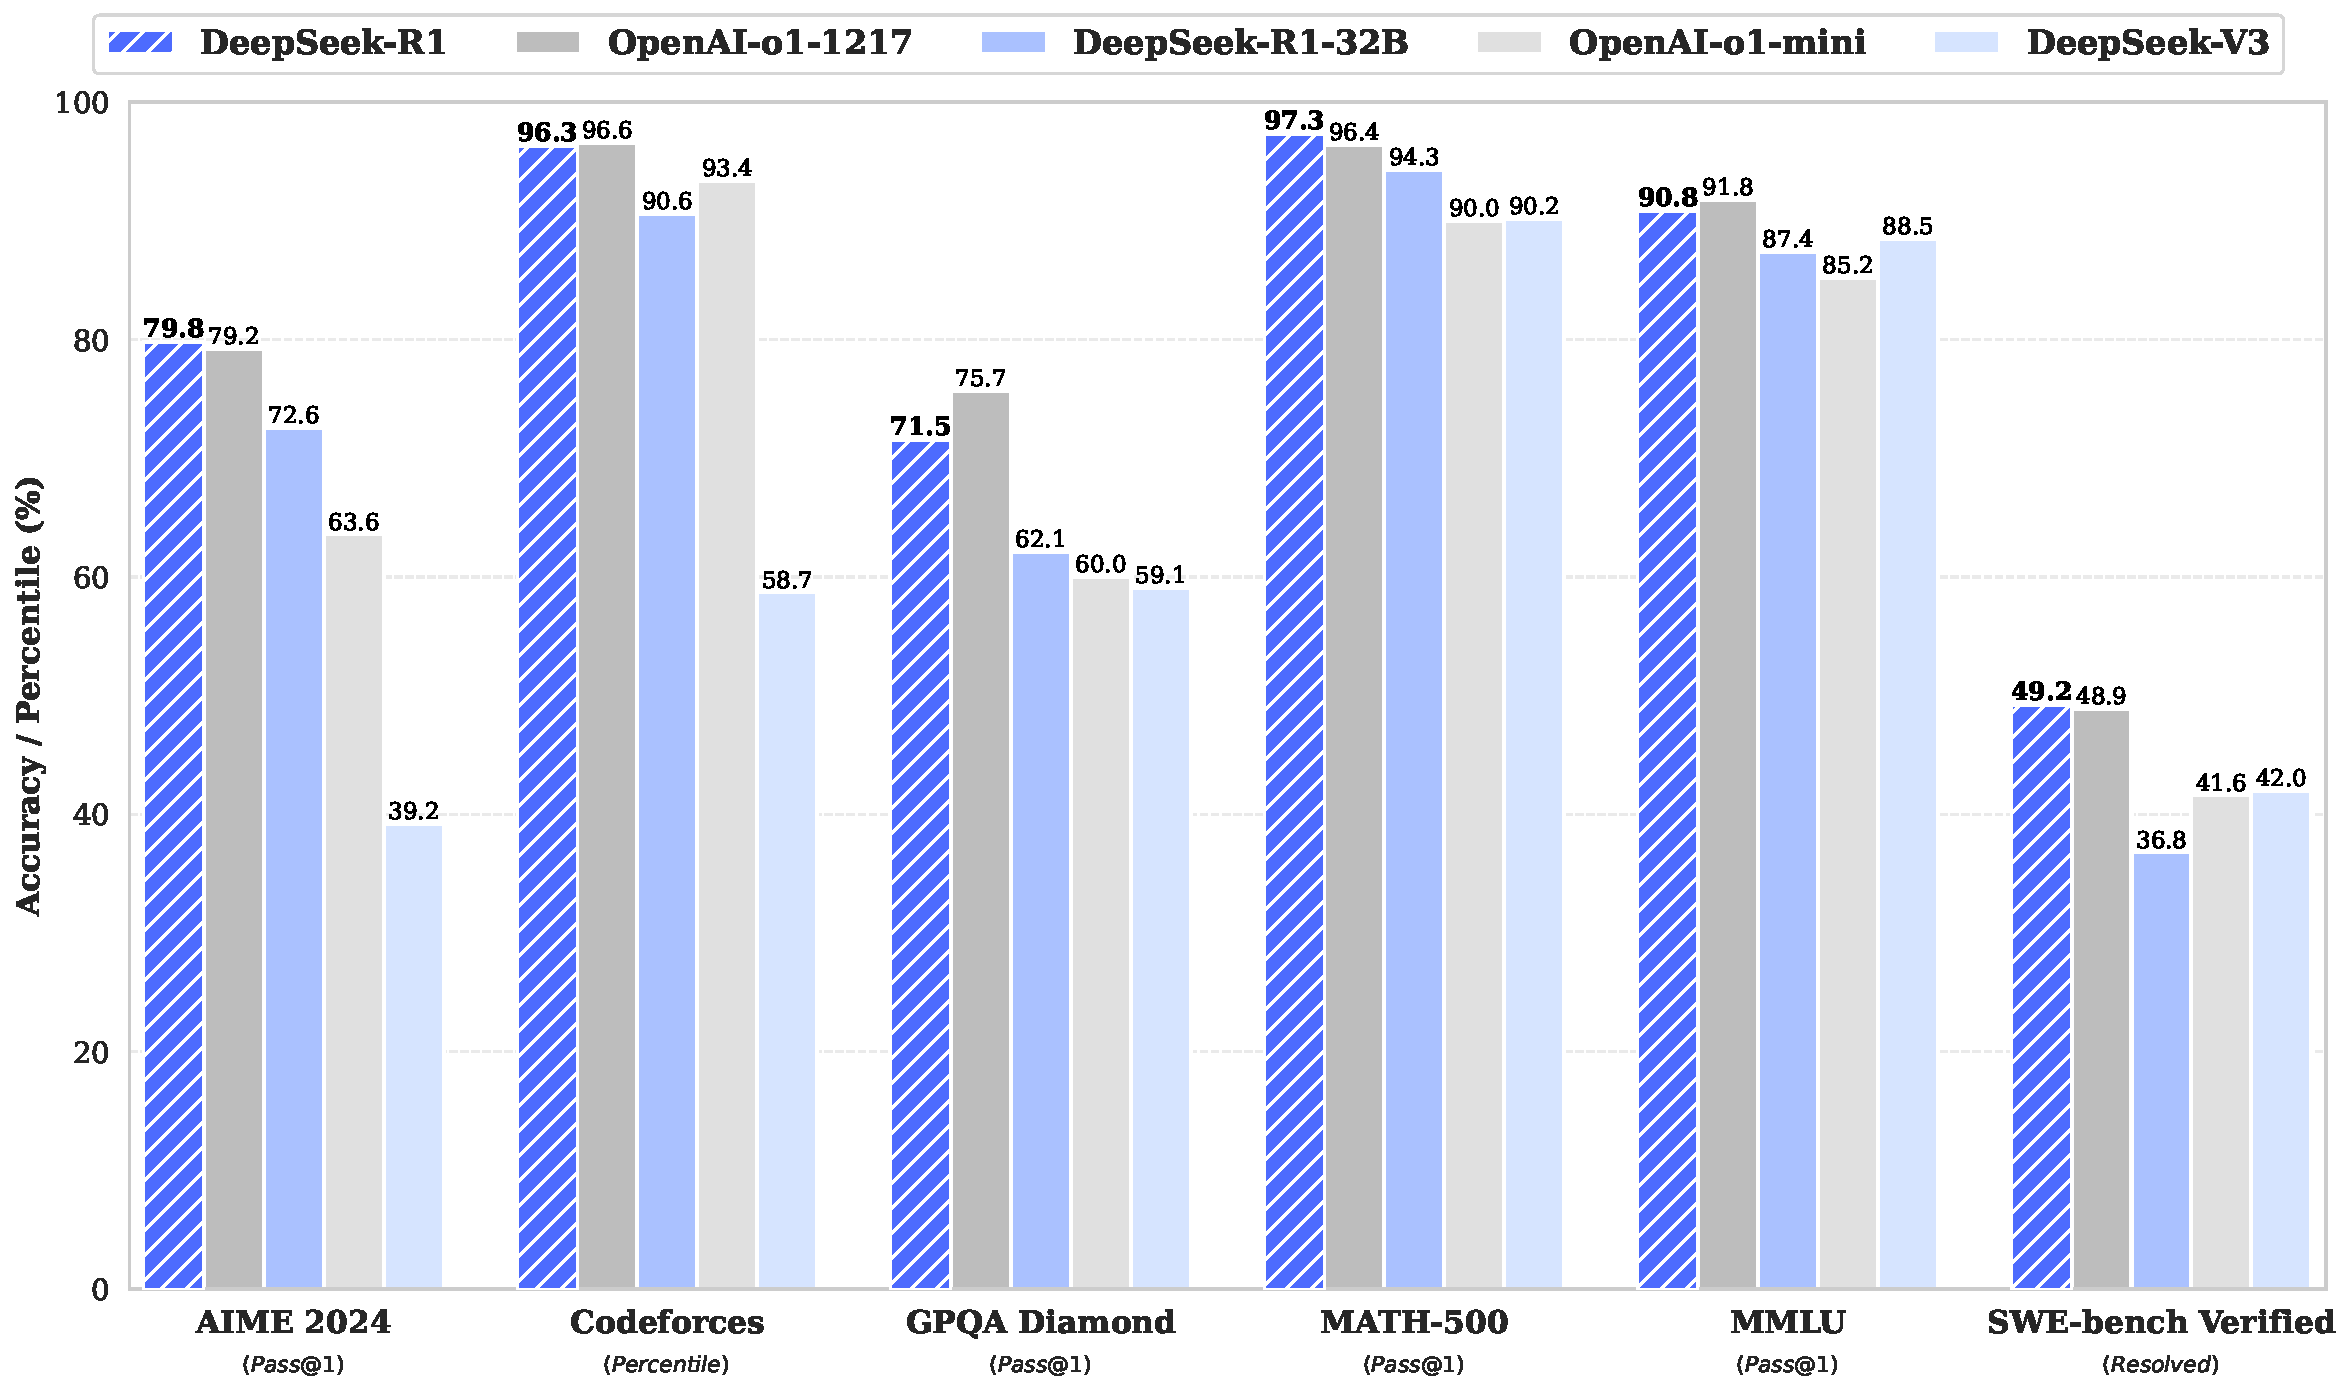
\includegraphics[width=1.0\textwidth]{figures/dsr1_performance.pdf}
\caption{
    \centering
    \dsri{} 的基准性能。
}
\label{fig:dsv3_performance}
\end{figure}

\newpage

\begin{spacing}{0.9}
\tableofcontents
\end{spacing}

\newpage
\section{介绍}
近年来,大型语言模型(LLMs)正在快速迭代和演化~\citep{gpt4o,claude35sonnet,gemini1_5},逐步缩小与人工通用智能(AGI)之间的差距。

最近,后训练已成为完整训练流程中的重要组成部分。研究表明,它在推理任务上提高了准确性,与社会价值观对齐,并适应用户偏好,同时与预训练相比需要相对较少的计算资源。在推理能力的背景下,OpenAI的o1~\citep{o1}系列模型率先通过增加思维链推理过程的长度引入了推理时间扩展。这种方法在各种推理任务中取得了显著的改进,如数学、编码和科学推理。然而,有效测试时间扩展的挑战仍然是研究界的一个未解问题。若干先前的工作探索了各种方法,包括基于过程的奖励模型\citep{uesato2022solving, lightman2023let,mathshepherd}、强化学习\citep{kumar2024training}和搜索算法,如蒙特卡罗树搜索和束搜索\citep{feng2024alphazeroliketreesearchguidelarge,xin2024deepseekproverv15harnessingproofassistant,AlphaGeometryTrinh2024}。然而,这些方法中没有一个能达到与OpenAI的o1系列模型相当的一般推理性能。

在本文中,我们首次尝试使用纯强化学习(RL)来提高语言模型的推理能力。我们的目标是探索LLMs在不使用任何监督数据的情况下,通过纯RL过程自我进化发展推理能力的潜力。具体而言,我们使用DeepSeek-V3-Base作为基础模型,并采用GRPO~\citep{deepseekmath}作为RL框架来提高模型在推理方面的表现。在训练过程中,\dsro{}自然涌现出许多强大而有趣的推理行为。经过数千次RL步骤,\dsro{}在推理基准上表现出超强性能。例如,AIME 2024的pass@1得分从15.6\%提高到71.0\%,并且通过多数投票,得分进一步提高到86.7\%,匹配OpenAI-o1-0912的表现。

然而,\dsro{}遇到了一些挑战,如可读性差和语言混合。为了应对这些问题并进一步提高推理性能,我们引入了\dsri{},该方法结合了少量的冷启动数据和多阶段训练流程。具体而言,我们首先收集数千条冷启动数据以微调DeepSeek-V3-Base模型。随后,我们执行类似于\dsro{}的推理导向RL。当RL过程接近收敛时,我们通过在RL检查点上进行拒绝采样创建新的SFT数据,并结合来自DeepSeek-V3的监督数据(如写作、事实问答和自我认知领域),然后重新训练DeepSeek-V3-Base模型。在使用新数据微调后,检查点经历了额外的RL过程,考虑到所有场景的提示。经过这些步骤,我们获得了一个称为\dsri{}的检查点,其性能可与OpenAI-o1-1217媲美。

我们进一步探索了从\dsri{}到更小密集模型的蒸馏。以Qwen2.5-32B~\citep{qwen2_5}作为基础模型,直接从\dsri{}进行蒸馏优于在其上应用RL。这表明较大基础模型发现的推理模式对于提高推理能力至关重要。我们开源了蒸馏的Qwen和Llama~\citep{llama3}系列。值得注意的是,我们的蒸馏14B模型远远优于最先进的开源QwQ-32B-Preview~\citep{QwQ},而蒸馏的32B和70B模型在密集模型中的推理基准上创下了新纪录。
\subsection{贡献}

\paragraph{后训练:在基础模型上进行大规模强化学习}
\begin{itemize}[topsep=0pt]
    \item
    我们直接将强化学习(RL)应用于基础模型,而不依赖监督微调(SFT)作为初步步骤。这种方法使得模型可以探索思维链(CoT)来解决复杂问题,最终开发出 \dsro{}。\dsro{} 展现了自我验证、反思和生成长思维链等能力,标志着研究界的一个重大里程碑。值得注意的是,这是首次开放研究验证了大型语言模型(LLM)的推理能力可以完全通过RL激励实现,而无需SFT。这一突破为未来在该领域的发展铺平了道路。
    \item
    我们介绍了开发 \dsri{} 的流程。该流程包含两个RL阶段,旨在发现更好的推理模式并与人类偏好对齐,还有两个SFT阶段,作为模型推理和非推理能力的种子。我们相信这个流程将通过创造更好的模型为行业带来益处。

\end{itemize}

\paragraph{蒸馏:小模型也可以很强大}
\begin{itemize}[topsep=0pt]
    \item 我们证明了较大模型的推理模式可以被蒸馏到较小模型中,从而获得比通过RL在小模型上发现的推理模式更好的性能。开放源码的\dsri{}及其API将有助于研究社区在未来蒸馏出更好的小模型。
    \item 使用\dsri{}生成的推理数据,我们微调了几个研究社区广泛使用的密集模型。评估结果表明,蒸馏出的较小密集模型在基准测试中表现异常出色。DeepSeek-R1-Distill-Qwen-7B在AIME 2024上取得了55.5\%的成绩,超过了QwQ-32B-Preview。此外,DeepSeek-R1-Distill-Qwen-32B在AIME 2024上得分72.6\%,在MATH-500上得分94.3\%,在LiveCodeBench上得分57.2\%。这些结果显著优于先前的开源模型,并且与o1-mini相当。我们将基于Qwen2.5和Llama3系列的蒸馏1.5B、7B、8B、14B、32B和70B的检查点向社区开源。
\end{itemize}
\subsection{评估结果总结}
\begin{itemize}[topsep=0pt]

    \item \textbf{推理任务}:
    (1)
    \dsri{} 在 AIME 2024 上的 Pass@1 得分为 79.8\%,略微超越了 OpenAI-o1-1217。在 MATH-500 上,它取得了 97.3\% 的优异成绩,与 OpenAI-o1-1217 表现相当,并显著超过其他模型。
    (2)
    在与编码相关的任务中,\dsri{} 在代码竞赛任务中展示了专家级水平,Codeforces 的 Elo 评分为 2,029,超过了 96.3\% 的人类参赛者。在工程相关任务中,\dsri{} 的表现略优于 DeepSeek-V3,这可能有助于开发人员在实际任务中使用。

    \item \textbf{知识}:
    在 MMLU、MMLU-Pro 和 GPQA Diamond 等基准测试中,\dsri{} 取得了卓越的成绩,显著超过了 DeepSeek-V3,在 MMLU 上得分为 90.8\%,在 MMLU-Pro 上得分为 84.0\%,在 GPQA Diamond 上得分为 71.5\%。虽然在这些基准测试上的表现略低于 OpenAI-o1-1217,但 \dsri{} 超过了其他闭源模型,显示了其在教育任务中的竞争优势。在事实基准测试 SimpleQA 上,\dsri{} 的表现优于 DeepSeek-V3,展示了其处理基于事实的查询的能力。在这个基准测试上,OpenAI-o1 的表现也超过了 4o。
    \item \textbf{其他}:\dsri{} 还在广泛的任务中表现出色,包括创意写作、一般问答、编辑、摘要等。在 AlpacaEval 2.0 中,它取得了 87.6\% 的长度控制胜率,在 ArenaHard 中取得了 92.3\% 的胜率,展示了其智能处理非考试导向查询的强大能力。此外,\dsri{} 在需要长上下文理解的任务中表现出色,在长上下文基准测试中显著超过了 DeepSeek-V3。
\end{itemize}
\section{方法}
\subsection{概述}
之前的工作在很大程度上依赖于大量监督数据来提升模型性能。在这项研究中,我们展示了即使不使用监督微调(SFT)作为冷启动,通过大规模强化学习(RL)也可以显著提高推理能力。此外,通过包含少量冷启动数据可以进一步增强性能。在接下来的部分中,我们介绍:(1) \dsro{},它在没有任何 SFT 数据的情况下直接将 RL 应用于基础模型,(2) \dsri{},它从经过数千个长链式思维(CoT)示例微调的检查点开始应用 RL,(3) 将 \dsri{} 的推理能力提炼到小型密集模型中。
\subsection{ \dsro{}: 基于模型的强化学习}
\label{sec:ds-zero}
强化学习在推理任务中展示了显著的效果,这在我们之前的研究中得到了证实 \citep{mathshepherd,deepseekmath}。
然而,这些研究严重依赖于监督数据,而这些数据的收集需要大量时间。
在本节中,我们探讨大型语言模型在\textbf{没有任何监督数据}情况下发展推理能力的潜力,重点关注其通过纯粹的强化学习过程的自我进化。
我们首先简要概述我们的强化学习算法,然后展示一些激动人心的结果,并希望这能为学术界提供宝贵的见解。
\subsubsection{强化学习算法}
\paragraph{群体相对策略优化} 为了节省强化学习的训练成本,我们采用群体相对策略优化(GRPO) \citep{deepseekmath},该方法放弃了通常与策略模型大小相同的评论模型,而是从群体分数中估计基线。
具体而言,对于每个问题 $q$,GRPO 从旧策略 $\pi_{\theta_{old}}$ 中采样一组输出 $\{o_1, o_2, \cdots, o_G\}$,然后通过最大化以下目标来优化策略模型 $\pi_{\theta}$:
\begin{equation}
\begin{split}
    \mathcal{J}_{GRPO}(\theta) &= \mathbb{E}{[q \sim P(Q), \{o_i\}_{i=1}^G \sim \pi_{\theta_{old}}(O|q)]}  \\
    & \frac{1}{G}\sum_{i=1}^G \left( \min \left( \frac{\pi_\theta(o_i |q)}{\pi_{\theta_{old}}(o_i |q)} A_i, \text{clip} \left( \frac{\pi_\theta(o_i |q)}{\pi_{\theta_{old}}(o_i |q)}, 1 - \epsilon, 1 + \epsilon \right)  A_i \right) - \beta \mathbb{D}_{KL}\left(\pi_{\theta} || \pi_{ref}\right)\right) ,
\end{split}
\label{eq:GRPO-obj}
\end{equation}
\begin{equation}
    \mathbb{D}_{KL}\left(\pi_{\theta} || \pi_{ref}\right) = \frac{\pi_{ref}(o_i|q)}{\pi_{\theta}(o_i|q)}- \log\frac{\pi_{ref}(o_i|q)}{\pi_{\theta}(o_i|q)} - 1,
\end{equation}
其中 $\epsilon$ 和 $\beta$ 是超参数,$A_i$ 是优势,通过一组对应于每组输出的奖励 $\{r_1, r_2, \ldots, r_G\}$ 计算得到:
\begin{equation}
    A_i = \frac{r_i - {\mathrm mean(\{r_1, r_2, \cdots, r_G\})}}{{\mathrm std(\{r_1, r_2, \cdots, r_G\})}}.
\end{equation}

\begin{table}[t]
    \centering
    \small
    \begin{tabular}{l}
    \toprule
    A conversation between User and Assistant. The user asks a question, and the Assistant solves it. \\
     The assistant first thinks about the reasoning process in the mind and then provides the user \\ with the answer.
     The reasoning process and answer are enclosed within <think> </think> and \\<answer> </answer> tags, respectively, i.e., <think> reasoning process here </think> \\ <answer> answer here </answer>.
     User: \textcolor{red}{prompt}. Assistant: \\
     \bottomrule
    \end{tabular}
    \caption{ \dsro{} 的模板。 \textcolor{red}{prompt} 将在训练中被特定的推理问题替换。}
    \label{tab:r0_template}
\end{table}
\subsubsection{奖励建模} 奖励是训练信号的来源,决定了强化学习的优化方向。为了训练 \dsro{},我们采用了一种基于规则的奖励系统,主要由两种类型的奖励组成:
\begin{itemize}[topsep=0pt]
    \item \textbf{准确性奖励}: 准确性奖励模型评估响应是否正确。例如,对于具有确定性结果的数学问题,模型需要以指定格式(例如,在框内)提供最终答案,从而实现可靠的基于规则的正确性验证。同样,对于 LeetCode 问题,可以使用编译器根据预定义的测试用例生成反馈。
    \item \textbf{格式奖励}: 除了准确性奖励模型外,我们还使用格式奖励模型,强制模型将其思维过程放在 `<think>' 和 `</think>' 标签之间。
\end{itemize}
我们在开发 \dsro{} 时没有应用结果或过程神经奖励模型,因为我们发现神经奖励模型在大规模强化学习过程中可能会遭遇奖励作弊,并且重新训练奖励模型需要额外的训练资源,复杂化了整个训练流程。
\subsubsection{训练模板}

为了训练 \dsro{},我们首先设计了一个简单的模板,引导基础模型遵循我们指定的指令。如表 \ref{tab:r0_template} 所示,该模板要求 \dsro{} 首先产生一个推理过程,然后给出最终答案。我们故意将约束限制在这种结构格式上,避免任何内容特定的偏见,例如强制反思性推理或促进特定问题解决策略,以确保我们能够准确观察模型在强化学习过程中的自然进展。
\subsubsection{\dsro{} 的性能、自我进化过程和顿悟时刻}

\paragraph{\dsro{} 的性能}

\begin{table}[t]
    \centering
    \resizebox{\linewidth}{!}{
    \begin{tabular}{@{}l *{6}{c} @{}}
    \toprule
    \multirow{3}{*}{\centering\textbf{Model}} & \multicolumn{2}{c}{\multirow{2}{*}{\textbf{AIME 2024}}} & \multirow{2}{*}{\textbf{MATH-500}} & \textbf{GPQA} & \textbf{LiveCode} & \multirow{2}{*}{\textbf{CodeForces}} \\
     &  & &  & \textbf{Diamond} & \textbf{Bench} \\
    \cmidrule(lr){2-3}
     & pass@1 & cons@64 & pass@1 &  pass@1 & pass@1 & rating \\
    \midrule
    \textbf{OpenAI-o1-mini} & 63.6 & 80.0 & 90.0  & 60.0 & 53.8 & 1820 \\
    \textbf{OpenAI-o1-0912} & 74.4  & 83.3  & 94.8  & 77.3 & 63.4 & 1843 \\
    \midrule
    \textbf{\dsro{}} & 71.0 & 86.7 & 95.9 & 73.3 & 50.0 & 1444 \\
    \bottomrule
    \end{tabular}
    }
    \caption{在推理相关基准测试中 \dsro{} 和 OpenAI o1 模型的比较。}
    \label{tab:r1-zero}
\end{table}

\begin{figure}
    \centering
    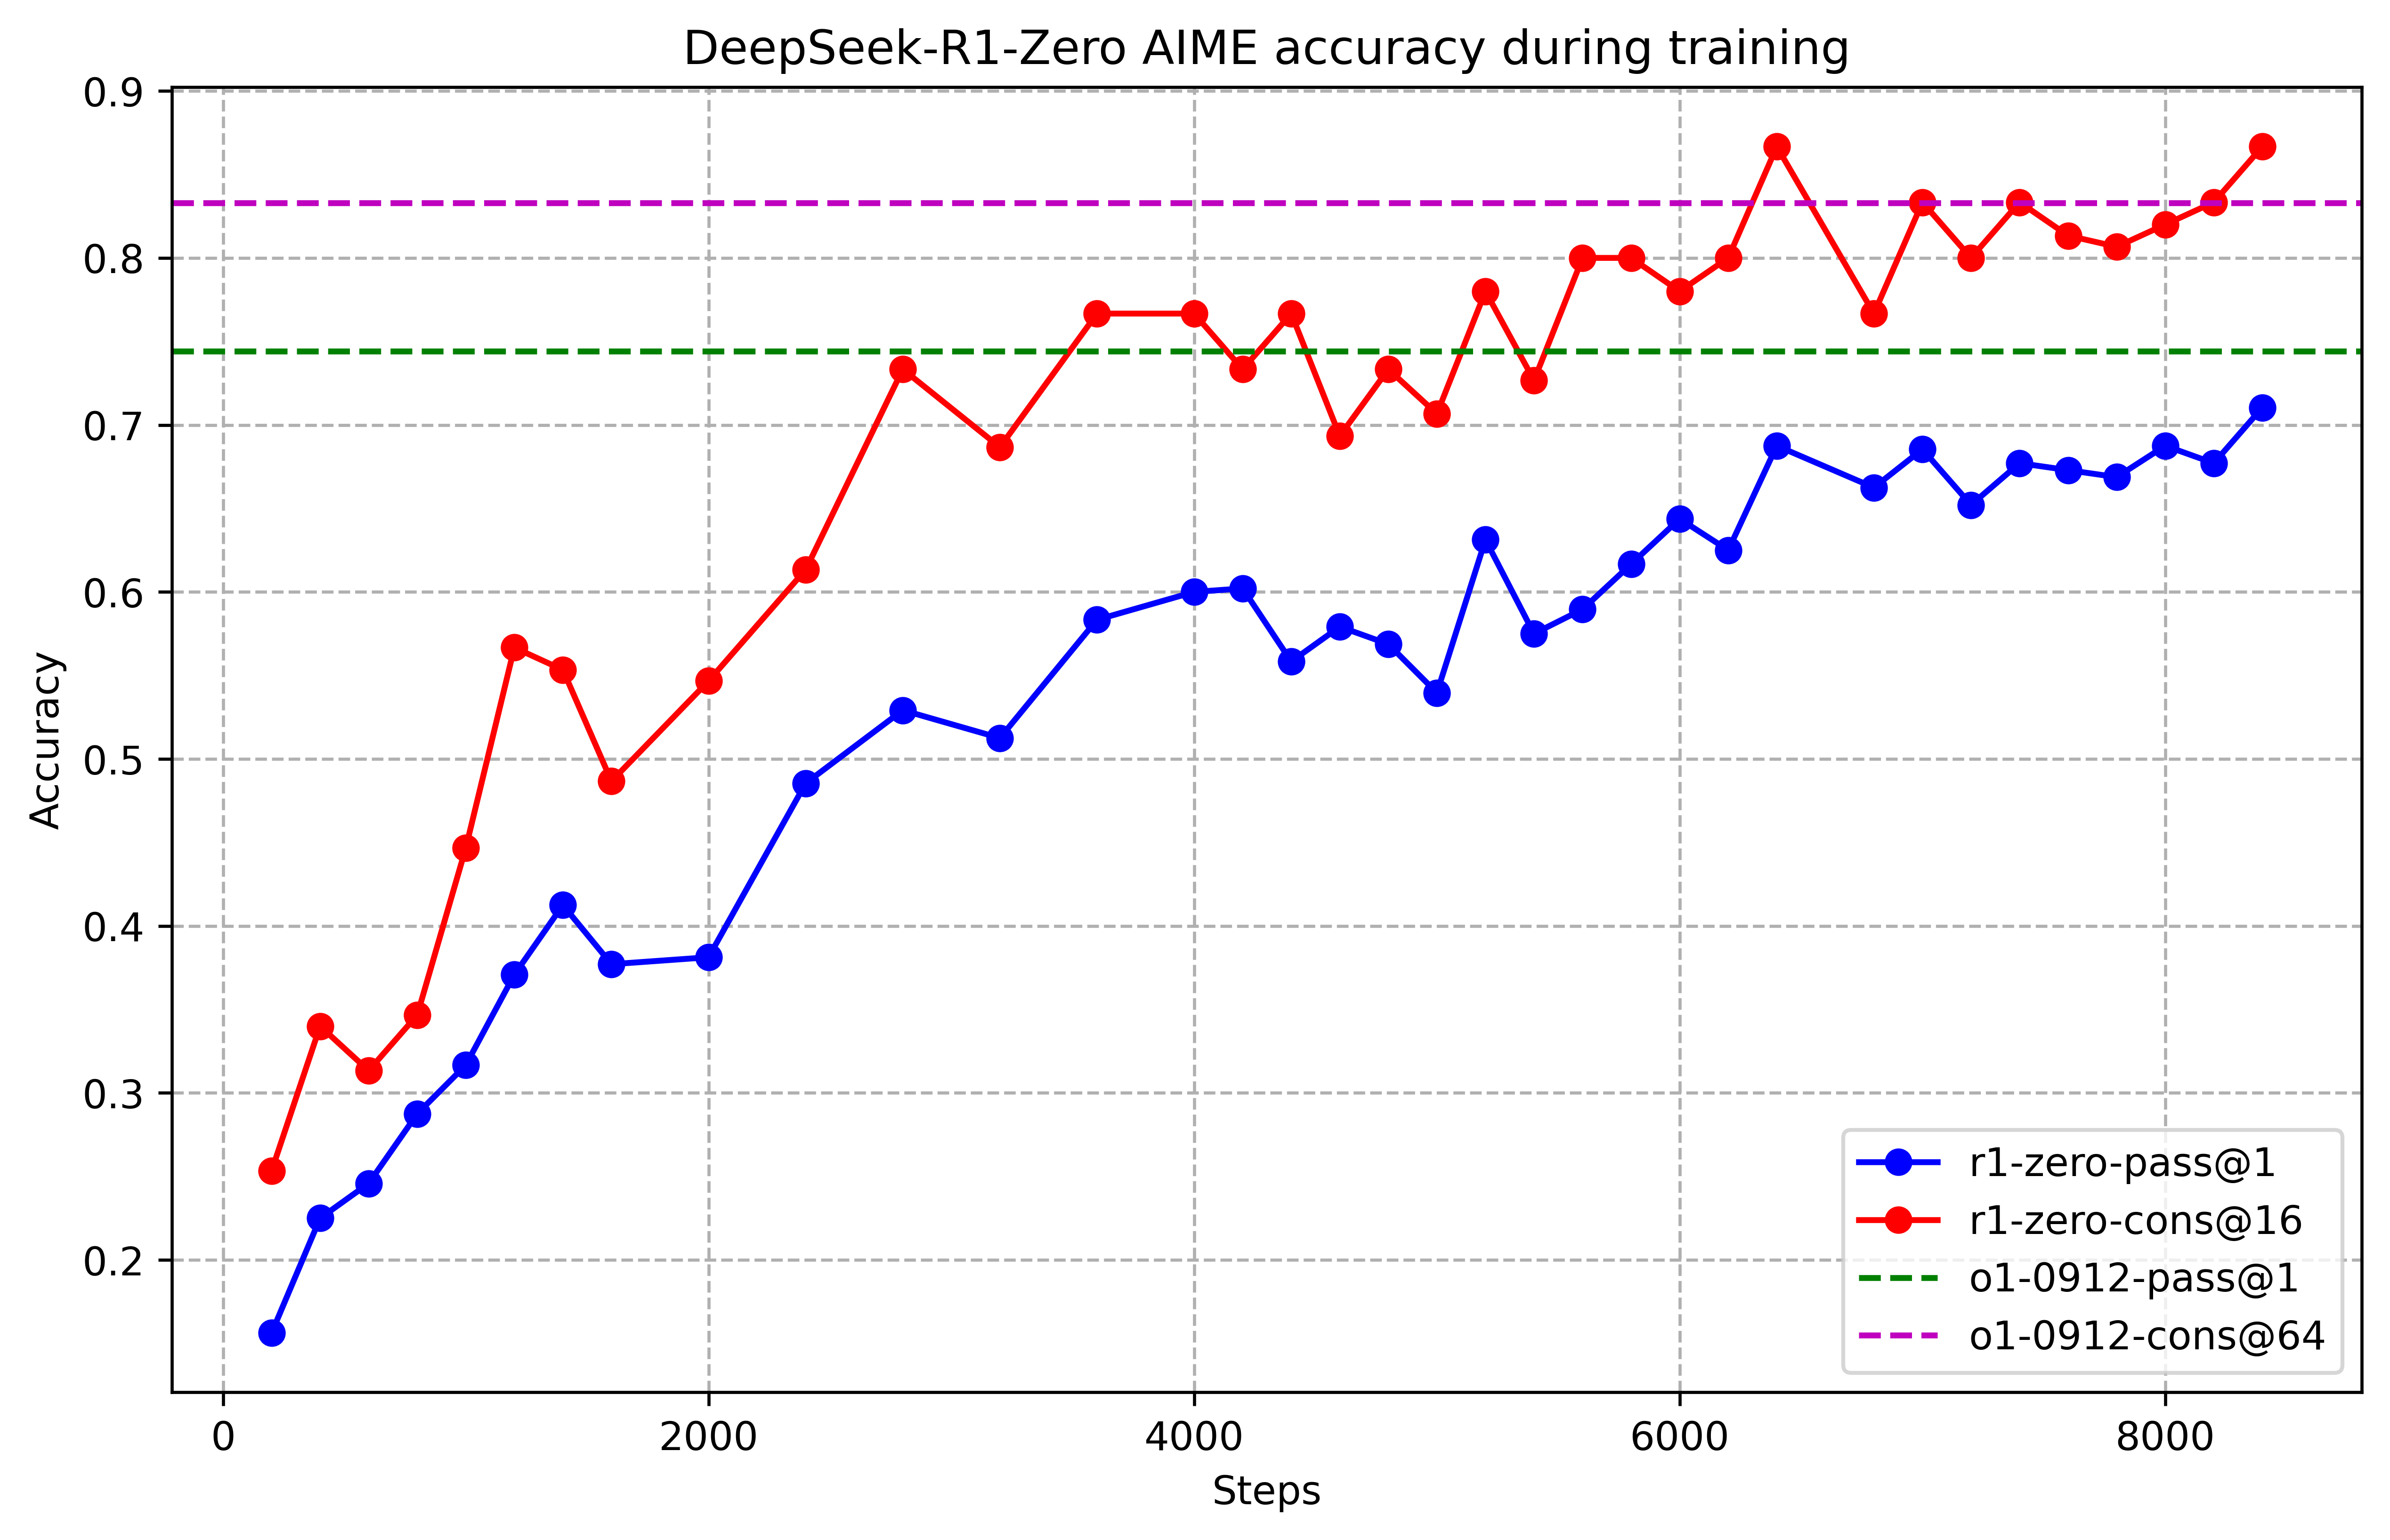
\includegraphics[width=0.75\linewidth]{figures/plot_aime_with_maj.png}
    \caption{\dsro{} 在训练期间的 AIME 准确性。对于每个问题,我们采样 16 个回答并计算总体平均准确性,以确保评估的稳定性。}
    \label{fig:zero-training-performance}
\end{figure}

图 \ref{fig:zero-training-performance} 描绘了 \dsro{} 在整个 RL 训练过程中在 AIME 2024 基准测试上的性能轨迹。如图所示,随着 RL 训练的推进,\dsro{} 的性能表现出稳定而一致的提升。值得注意的是,AIME 2024 的平均 pass@1 分数显著增加,从最初的 15.6\% 跃升至令人印象深刻的 71.0\%,达到了与 OpenAI-o1-0912 相当的性能水平。这一显著提升突出了我们 RL 算法在优化模型性能方面的有效性。

表 \ref{tab:r1-zero} 提供了 \dsro{} 与 OpenAI 的 o1-0912 模型在各种推理相关基准测试上的比较分析。研究结果表明,RL 使 \dsro{} 能够在无需任何监督微调数据的情况下实现强大的推理能力。这是一个值得注意的成就,因为它强调了模型通过 RL 单独学习和有效泛化的能力。此外,\dsro{} 的性能可以通过应用多数投票进一步增强。例如,当在 AIME 基准测试上采用多数投票时,\dsro{} 的性能从 71.0\% 上升到 86.7\%,从而超过了 OpenAI-o1-0912 的性能。
\dsro{} 能够在有无多数投票的情况下实现如此竞争力的表现,突出了其强大的基础能力及其在推理任务中进一步进步的潜力。

\begin{figure}[t]
    \centering
    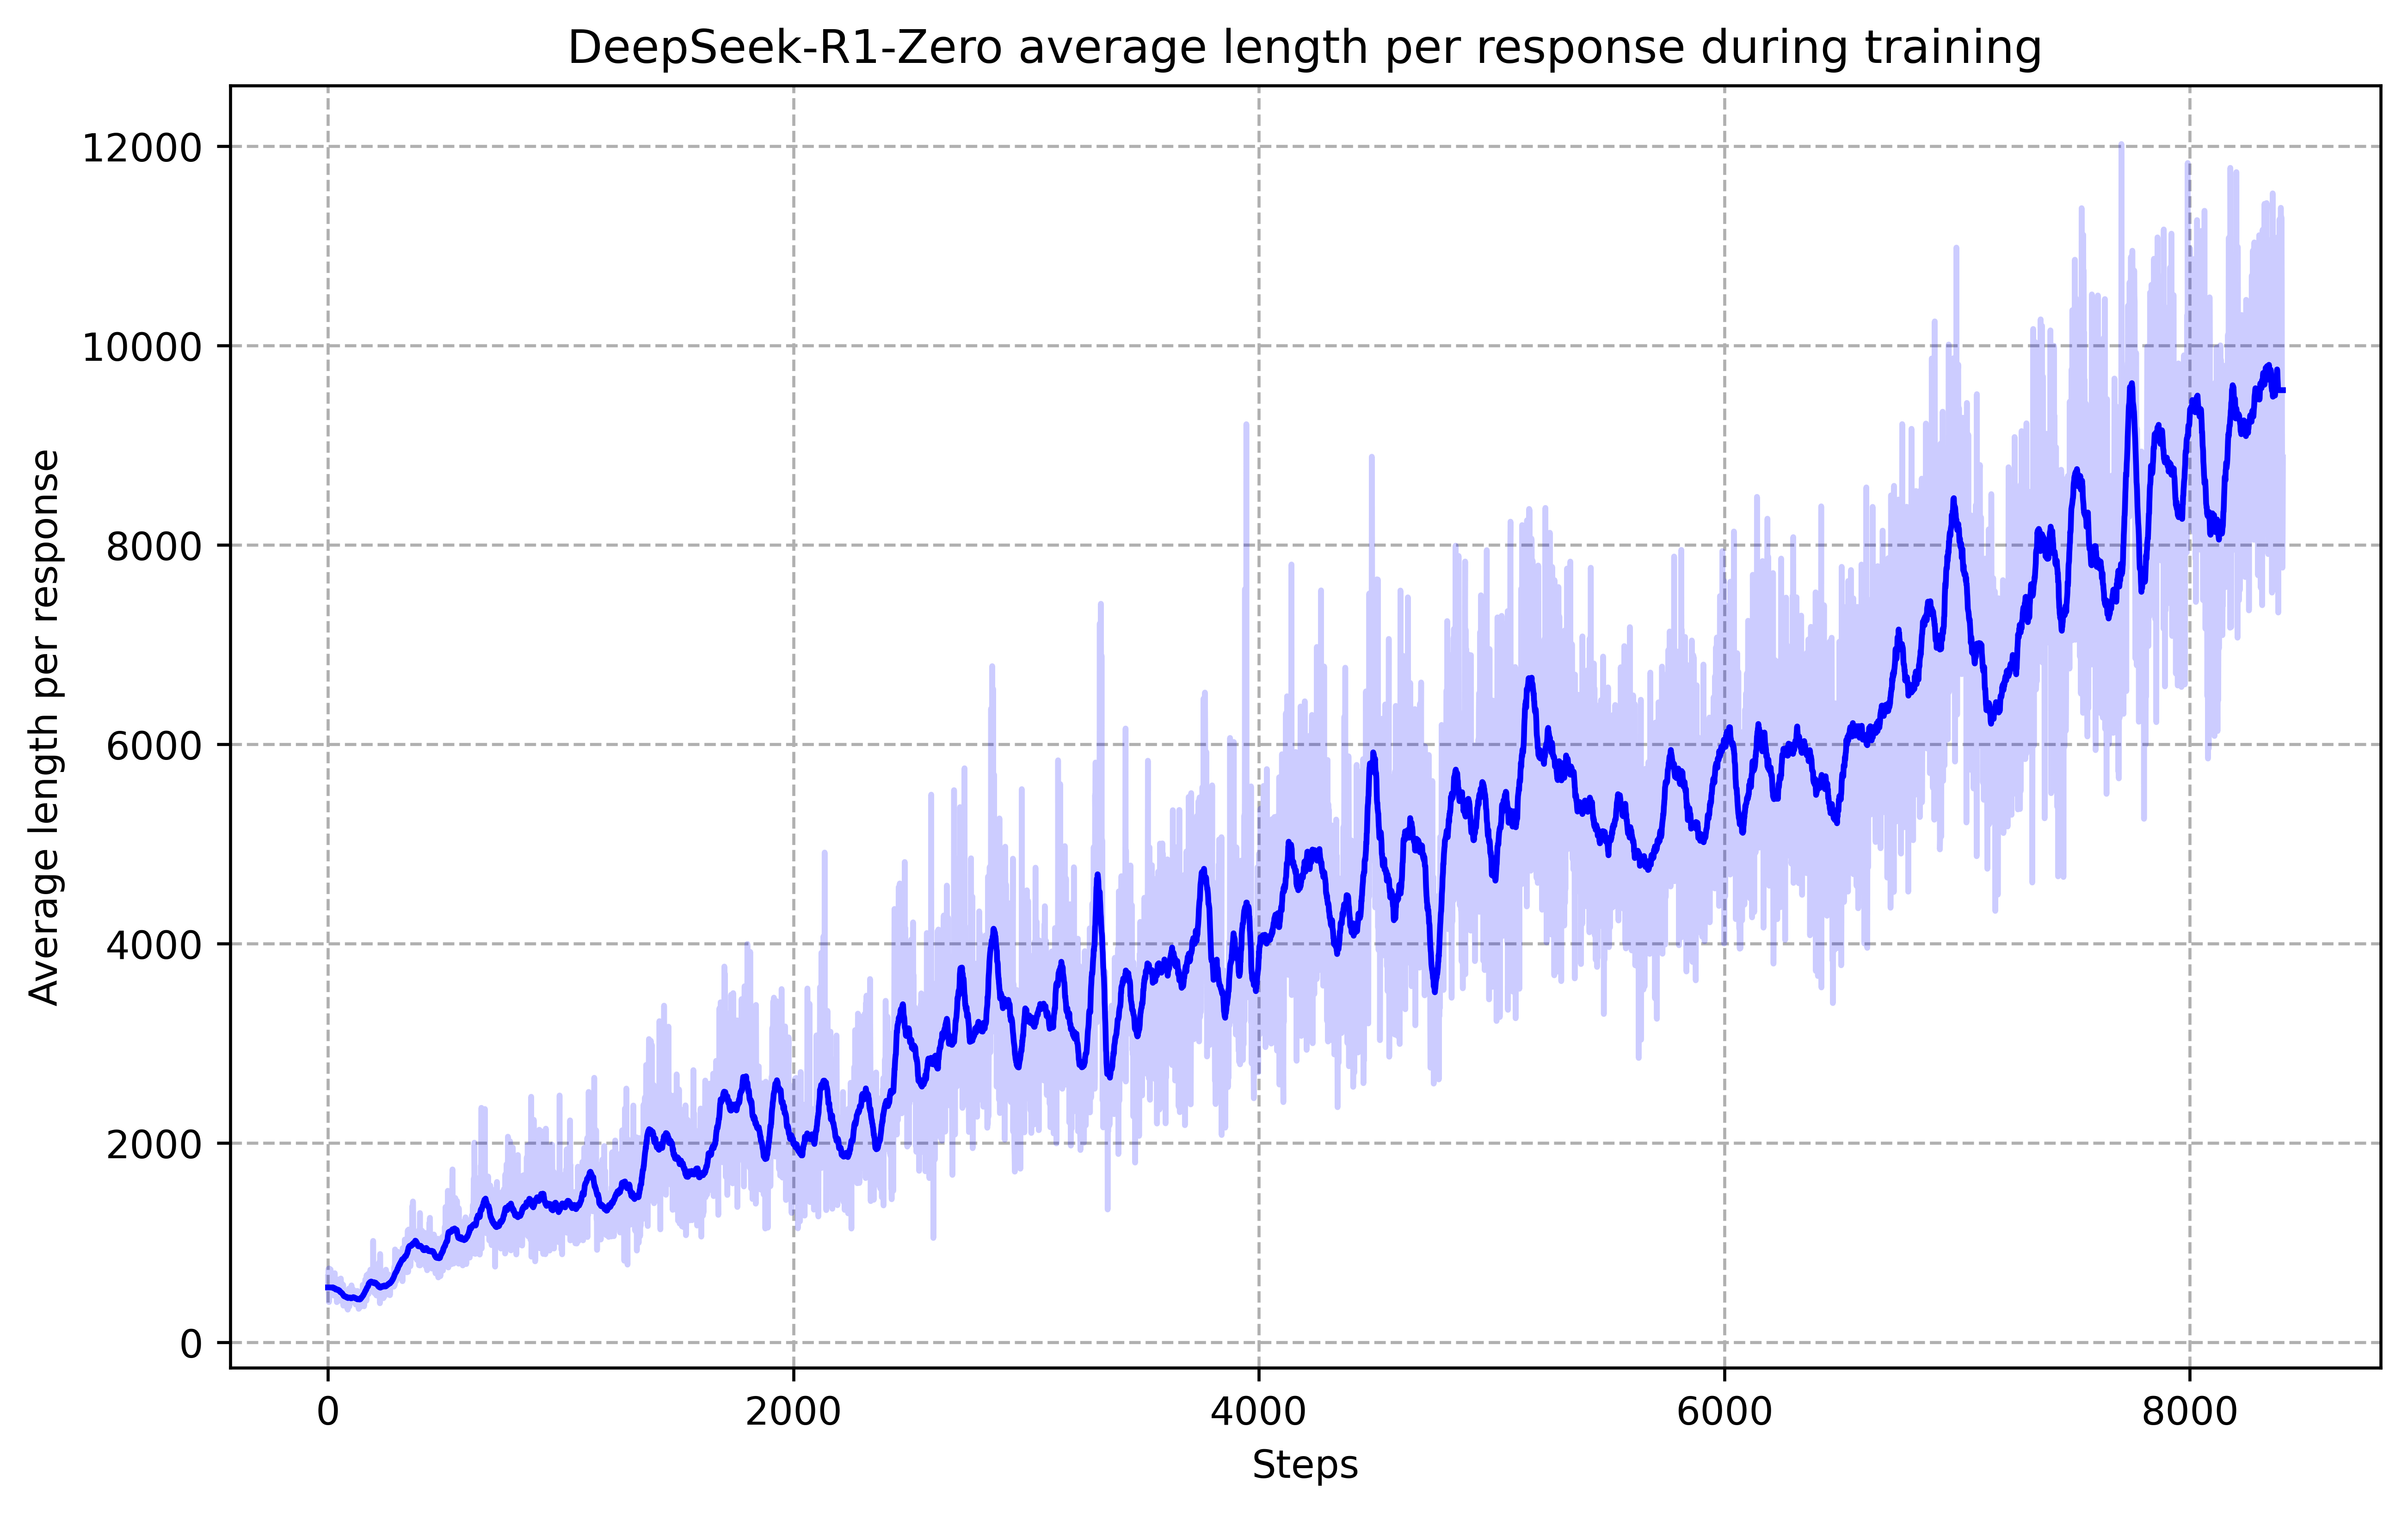
\includegraphics[width=0.75\linewidth]{figures/plot_length.png}
    \caption{\dsro{} 在训练集上的平均响应长度在 RL 过程中的变化。 \dsro{} 自然地学习在推理任务中使用更多的思考时间。}
    \label{fig:zero-training-length}
\end{figure}

\paragraph{\dsro{} 的自我进化过程}
\dsro{} 的自我进化过程是一个引人入胜的示范,展示了 RL 如何驱动模型自主改善其推理能力。通过直接从基础模型启动 RL,我们可以在没有监督微调阶段影响的情况下密切监测模型的进展。此方法提供了对模型随时间演变的清晰视角,尤其是在处理复杂推理任务的能力方面。

如图 \ref{fig:zero-training-length} 所示,\dsro{} 的思考时间在整个训练过程中显示出持续改进。这种改进并非外部调整的结果,而是模型内在发展的结果。\dsro{} 自然地通过利用扩展的测试时间计算来获取解决日益复杂推理任务的能力。这种计算范围从生成数百到数千个推理符号,使模型能够更深入地探索和完善其思考过程。

这种自我进化最显著的方面之一是随着测试时间计算的增加而出现的复杂行为。诸如反思——模型重新审视并重新评估其先前步骤——以及探索替代问题解决方法等行为自发出现。这些行为不是明确编程的,而是模型与强化学习环境互动的结果。这种自发发展显著增强了 \dsro{} 的推理能力,使其能够更高效、更准确地应对更具挑战性的任务。

\paragraph{\dsro{} 的顿悟时刻}
在 \dsro{} 的训练过程中观察到的一个特别引人入胜的现象是“顿悟时刻”的出现。这个时刻,如表 \ref{tab:aha_moment} 所示,发生在模型的中间版本。在此阶段,\dsro{} 通过重新评估其初始方法来学习为问题分配更多思考时间。这种行为不仅是模型推理能力增强的证明,也是一个迷人的例子,展示了强化学习如何导致意想不到和复杂的结果。

这一时刻不仅是模型的“顿悟时刻”,也是研究人员观察其行为的“顿悟时刻”。它强调了强化学习的力量和美丽:我们不是明确教导模型如何解决问题,而只是为其提供正确的激励,它就会自主开发高级问题解决策略。
“顿悟时刻”是一个强有力的提醒,展示了 RL 解锁人工系统新智能水平的潜力,为未来更自主和适应性更强的模型铺平了道路。

\paragraph{\dsro{} 的缺陷}
尽管 \dsro{} 展现了强大的推理能力,并自主开发了意想不到且强大的推理行为,它仍面临几个问题。例如,\dsro{} 的挑战包括可读性差以及语言混合。为了使推理过程更具可读性并与开放社群分享,我们探索了 \dsri{},这是一种利用 RL 与人类友好冷启动数据的方法。

\begin{table}[t]
\centering
\begin{tabular}{l}
\toprule
Question: If \(a > 1\), then the sum of the real solutions of \(\sqrt{a - \sqrt{a + x}} = x\) is equal to \\
\midrule
Response: <think> \\
To solve the equation \(\sqrt{a - \sqrt{a + x}} = x\), let's start by squaring both $\cdots$ \\
$\left(\sqrt{a - \sqrt{a + x}}\right)^2 = x^2 \implies a - \sqrt{a + x} = x^2.$ \\
Rearrange to isolate the inner square root term: \\
$(a - x^2)^2 = a + x \implies a^2 - 2ax^2 + (x^2)^2 = a + x \implies x^4 - 2ax^2 - x + (a^2 - a) = 0$ \\
\ldots \\
\textcolor{red}{Wait, wait. Wait. That's an aha moment I can flag here}. \\
Let's reevaluate this step-by-step to identify if the correct sum can be $\cdots$ \\
We started with the equation: \\
$\sqrt{a - \sqrt{a + x}} = x$ \\
First, let's square both sides: \\
$a - \sqrt{a + x} = x^2 \implies \sqrt{a + x} = a - x^2$ \\
Next, I could square both sides again, treating the equation:
$\cdots$
\\
\ldots \\
\hline
\end{tabular}
\caption{一个有趣的 \dsro{} 中间版本的 ``aha 时刻''。模型学会用拟人化的语气重新思考。这对我们来说也是一个 aha 时刻,让我们见证了强化学习的力量和美妙。}
\label{tab:aha_moment}
\end{table}
\subsection{\dsri{}: 冷启动下的强化学习}
受益于\dsro{}的良好结果,我们自然会提出两个问题:1)通过引入少量高质量数据作为冷启动,能否进一步提高推理性能或加速收敛?2)我们如何训练一个不仅能生成清晰连贯的思维链(CoT),而且表现出强大通用能力的用户友好型模型?
为了解决这些问题,我们设计了一个用于训练\dsri{}的流程。该流程包括以下四个阶段。
\subsubsection{冷启动}
与 \dsro{} 不同,为了防止 RL 训练初期不稳定的冷启动阶段在基础模型中发生,对于 DeepSeek-R1,我们构建并收集少量长 CoT 数据以微调模型作为初始 RL actor。
为了收集这些数据,我们探索了几种方法:使用少量示例提示以长 CoT 作为例子,直接提示模型生成带有反思和验证的详细答案,以可读格式收集 \dsro{} 的输出,并通过人工注释者进行后处理以改进结果。

在这项工作中,我们收集了数千个冷启动数据以微调 DeepSeek-V3-Base 作为 RL 的起始点。
与 \dsro{} 相比,冷启动数据的优势包括:
\begin{itemize}[topsep=0pt]
    \item
可读性:\dsro{} 的一个关键限制是其内容通常不适合阅读。响应可能混合多种语言或缺乏用于突出显示用户答案的 markdown 格式。相比之下,在为 \dsri{} 创建冷启动数据时,我们设计了一种可读的模式,在每个响应末尾包括摘要,并过滤掉不易阅读的响应。在这里,我们将输出格式定义为 | special\_token| <reasoning\_process> | special\_token| <summary> ,其中推理过程是查询的 CoT,摘要用于总结推理结果。

 \item
潜力:通过精心设计具有人工先验的冷启动数据模式,我们观察到相较于 \dsro{} 的更好表现。我们相信迭代训练对于推理模型来说是更好的方式。
\end{itemize}
\subsubsection{面向推理的强化学习}
在对DeepSeek-V3-Base进行冷启动数据微调之后,我们应用与\dsro相同的大规模强化学习训练过程。此阶段重点在于增强模型的推理能力,特别是在推理密集型任务中,如编程、数学、科学和逻辑推理,这些任务涉及具有明确解决方案的明确定义的问题。在训练过程中,我们观察到当强化学习提示涉及多种语言时,CoT经常会出现语言混合。为缓解语言混合问题,我们在强化学习训练过程中引入了语言一致性奖励,该奖励计算为CoT中目标语言词汇的比例。尽管消融实验显示这种对齐会导致模型性能的轻微下降,但该奖励符合人类偏好,使其更具可读性。最后,我们通过直接相加推理任务的准确性和语言一致性奖励来形成最终奖励。然后,我们在微调的模型上应用强化学习训练,直到其在推理任务上达到收敛。
\subsubsection{拒绝采样与监督微调}
当面向推理的强化学习(RL)收敛时,我们利用所得的检查点收集下一轮的监督微调(SFT)数据。与最初的冷启动数据主要关注推理不同,这一阶段结合了其他领域的数据,以提升模型在写作、角色扮演和其他通用任务中的能力。具体而言,我们按照以下描述生成数据并微调模型。
\label{sec:method:r1:sft}

\paragraph{推理数据}
我们通过从上述RL训练的检查点执行拒绝采样来策划推理提示并生成推理轨迹。在前一阶段,我们仅包括可以使用基于规则的奖励进行评估的数据。然而,在这一阶段,我们通过加入额外的数据扩展了数据集,其中一些数据通过将真实值和模型预测输入DeepSeek-V3进行判断,使用生成的奖励模型。此外,由于模型输出有时混乱且难以阅读,我们过滤掉了使用混合语言、长段落和代码块的思维链。对于每个提示,我们采样多个响应并仅保留正确的响应。总共,我们收集了大约60万条与推理相关的训练样本。

\paragraph{非推理数据}
对于非推理数据,如写作、事实问答、自我认知和翻译,我们采用DeepSeek-V3管道并重用DeepSeek-V3的部分SFT数据集。对于某些非推理任务,我们调用DeepSeek-V3在回答问题前,通过提示生成潜在的思维链。然而,对于简单的查询,如“hello”,我们不提供思维链响应。最终,我们收集了大约20万条与推理无关的训练样本。

我们使用上述策划的数据集(约80万样本)对DeepSeek-V3-Base进行两次迭代的微调。
\subsubsection{所有场景的强化学习}

为了进一步使模型与人类偏好保持一致,我们实施了一个次级强化学习阶段,旨在提高模型的有用性和无害性,同时改进其推理能力。具体而言,我们使用奖励信号和多样化的提示分布的组合来训练模型。
对于推理数据,我们遵循 \dsro 中概述的方法,该方法利用基于规则的奖励来引导数学、代码和逻辑推理领域的学习过程。
对于一般数据,我们依靠奖励模型在复杂和细微的场景中捕捉人类偏好。我们在 DeepSeek-V3 管道的基础上,采用类似的偏好对和训练提示的分布。对于有用性,我们专注于最终总结,确保评估强调响应对用户的实用性和相关性,同时尽量减少对基础推理过程的干扰。对于无害性,我们评估模型的整个响应,包括推理过程和总结,以识别和减轻生成过程中可能出现的任何潜在风险、偏见或有害内容。
最终,奖励信号和多样化数据分布的整合使我们能够训练出在推理中表现出色,同时优先考虑有用性和无害性的模型。
\subsection{蒸馏:赋予小模型推理能力}

为了使更高效的小模型具备像 DeepSeek-R1 这样的推理能力,我们直接使用 DeepSeek-R1 精心挑选的 80 万个样本对开源模型如 Qwen \citep{qwen2_5} 和 Llama \citep{llama3_1_405b} 进行了微调,具体细节见 \S \ref{sec:method:r1:sft}。我们的研究结果表明,这种直接的蒸馏方法显著增强了小模型的推理能力。我们在此使用的基础模型包括 Qwen2.5-Math-1.5B、Qwen2.5-Math-7B、Qwen2.5-14B、Qwen2.5-32B、Llama-3.1-8B 和 Llama-3.3-70B-Instruct。我们选择 Llama-3.3 是因为其推理能力略优于 Llama-3.1。

对于蒸馏模型,我们仅应用 SFT 并不包括 RL 阶段,尽管结合 RL 可以显著提升模型性能。我们此处的主要目标是展示蒸馏技术的有效性,而将 RL 阶段的探索留给更广泛的研究社区。
\section{实验}

\paragraph{基准测试} 我们在 MMLU \citep{mmlu}, MMLU-Redux \citep{mmlu_redux}, MMLU-Pro \citep{mmlu_pro}, C-Eval \citep{ceval}, 和 CMMLU \citep{cmmlu}, IFEval~\citep{IFeval}, FRAMES~\citep{frames}, GPQA Diamond ~\citep{gpqa}, SimpleQA~\citep{simpleqa}, C-SimpleQA~\citep{csimpleqa}, SWE-Bench Verified~\citep{swe_verified}, Aider~\footnote{\url{https://aider.chat}}, LiveCodeBench~\citep{livecodebench} (2024-08 -- 2025-01), Codeforces~\footnote{\url{https://codeforces.com}}, 中国全国高中数学奥林匹克竞赛 (CNMO 2024)\footnote{\url{https://www.cms.org.cn/Home/comp/comp/cid/12.html}}, 和美国邀请数学考试 2024 (AIME 2024)~\citep{AIME2024} 上评估模型。 除了标准基准测试外,我们还使用 LLMs 作为评判者评估模型在开放式生成任务上的表现。具体而言,我们遵循 AlpacaEval 2.0~\citep{alpaca2.0} 和 Arena-Hard~\citep{li2024crowdsourced} 的原始配置,这些配置利用 GPT-4-Turbo-1106 作为成对比较的评判者。 在这里,我们仅将最终摘要输入评估以避免长度偏差。对于压缩模型,我们报告 AIME 2024、MATH-500、GPQA Diamond、Codeforces 和 LiveCodeBench 上的代表性结果。

\paragraph{评估提示} 按照 DeepSeek-V3 中的设置,MMLU、DROP、GPQA Diamond 和 SimpleQA 等标准基准测试使用 simple-evals 框架中的提示进行评估。对于 MMLU-Redux,我们在零样本设置中采用 Zero-Eval 提示格式~\citep{Lin_ZeroEval_A_Unified_2024}。至于 MMLU-Pro、C-Eval 和 CLUE-WSC,由于原始提示是少样本的,我们略微修改提示为零样本设置。少样本中的 CoT 可能会影响 \dsri{} 的性能。其他数据集遵循其创作者提供的默认提示的原始评估协议。对于代码和数学基准测试,HumanEval-Mul 数据集涵盖八种主流编程语言(Python、Java、C++、C\#、JavaScript、TypeScript、PHP 和 Bash)。 LiveCodeBench 的模型性能使用 CoT 格式进行评估,数据收集时间为 2024 年 8 月至 2025 年 1 月。Codeforces 数据集使用 10 场 Div.2 比赛的问题及专家设计的测试用例进行评估,然后计算预期评分和竞争者百分比。SWE-Bench 验证结果通过无代理框架~\citep{agentless} 获得。AIDER 相关基准使用“diff”格式进行测量。 \dsri{} 输出在每个基准上最多限制为 32,768 个标记。

\paragraph{基线} 我们对多个强大的基线进行了全面评估,包括 DeepSeek-V3、Claude-Sonnet-3.5-1022、GPT-4o-0513、OpenAI-o1-mini 和 OpenAI-o1-1217。由于在中国大陆访问 OpenAI-o1-1217 API 存在困难,我们根据官方报告记录其性能。对于压缩模型,我们还比较了开源模型 QwQ-32B-Preview \citep{QwQ}。

\paragraph{评估设置} 我们将模型的最大生成长度设置为 32,768 个标记。我们发现使用贪婪解码评估长输出推理模型会导致更高的重复率,并且在不同检查点之间存在显着的可变性。因此,我们默认使用 pass@$k$ 评估 \citep{codex} 并使用非零温度报告 pass@1。具体来说,我们使用采样温度 $0.6$ 和 top-$p$ 值 $0.95$ 来为每个问题生成 $k$ 个响应(通常在 $4$ 到 $64$ 之间,具体取决于测试集的大小)。然后计算 pass@1 如下
\[
\text{pass@1} = \frac{1}{k} \sum_{i=1}^{k} p_i,
\]
其中 $p_i$ 表示第 $i$ 个响应的正确性。此方法提供了更可靠的性能估计。对于 AIME 2024,我们还使用 $64$ 个样本报告共识(多数投票)结果 \citep{wang2022self},记为 $\text{cons}@64$。
\subsection{\dsri{} 评估}

\begin{table}[h]
    \centering
    \footnotesize
    \setlength{\tabcolsep}{1.9pt}
    \begin{tabular}{@{}c l | c  c  c | c c |c c@{}}
    \toprule
    & \multirow{2}{*}{\centering \textbf{Benchmark {\tiny (Metric)}}}  & \textbf{Claude-3.5-}  & \textbf{GPT-4o}& \textbf{DeepSeek} & \textbf{OpenAI} & \textbf{OpenAI} & \textbf{DeepSeek}\\
    & & \textbf{Sonnet-1022}  & \textbf{0513} & \textbf{V3} & \textbf{o1-mini}& \textbf{o1-1217} &\textbf{R1} \\
    \midrule
    & Architecture &-&- & MoE &-&-& MoE \\
    & \# Activated Params& -&-& 37B&-&- & 37B \\
    & \# Total Params &-&-& 671B&-&- & 671B \\
    \midrule
    \multirow{10}{*}{English}& MMLU {\tiny (Pass@1)} & 88.3&87.2 & 88.5 & 85.2 & \textbf{91.8} & 90.8\\
     & MMLU-Redux {\tiny (EM)}& 88.9& 88.0 & 89.1 & 86.7&- & \textbf{92.9} \\
    & MMLU-Pro {\tiny (EM)}  & 78.0 & 72.6 & 75.9 & 80.3 &-& \textbf{84.0} \\
    & DROP {\tiny (3-shot F1)}  & 88.3 & 83.7 & 91.6 & 83.9 & 90.2 & \textbf{92.2}\\
    & IF-Eval {\tiny (Prompt Strict)}  & \textbf{86.5} & 84.3 & 86.1 & 84.8&- & 83.3 \\
    & GPQA Diamond {\tiny (Pass@1)}& 65.0 & 49.9 & 59.1 & 60.0 & \textbf{75.7} & 71.5&  \\
    & SimpleQA {\tiny (Correct)} & 28.4 & 38.2& 24.9 & 7.0 & \textbf{47.0} & 30.1 \\
     & FRAMES {\tiny (Acc.)}  & 72.5 & 80.5 & 73.3 & 76.9 & -&\textbf{82.5}\\
      & AlpacaEval2.0 {\tiny (LC-winrate)}  & 52.0 &  51.1 & 70.0 & 57.8 & - & \textbf{87.6}\\
       & ArenaHard {\tiny (GPT-4-1106)}  & 85.2 & 80.4 & 85.5 & 92.0 & - & \textbf{92.3}\\
    \midrule
    \multirow{4}{*}{Code} & LiveCodeBench {\tiny (Pass@1-COT)} & 38.9 & 32.9 & 36.2 & 53.8 & 63.4 & \textbf{65.9} \\
    & Codeforces {\tiny (Percentile)}& 20.3 & 23.6 & 58.7 & 93.4 & \textbf{96.6} & 96.3 \\
    & Codeforces {\tiny (Rating)}& 717 & 759 & 1134 & 1820 & \textbf{2061} & 2029 \\
    & SWE Verified {\tiny (Resolved)} & \textbf{50.8}&38.8&42.0 & 41.6 & 48.9 & 49.2\\
    & Aider-Polyglot {\tiny (Acc.)} & 45.3&16.0& 49.6 & 32.9 & \textbf{61.7}&53.3\\
    \midrule
    \multirow{3}{*}{Math} & AIME 2024 {\tiny (Pass@1)}  & 16.0 & 9.3 & 39.2 & 63.6 & 79.2 & \textbf{79.8} \\
    & MATH-500 {\tiny (Pass@1)} &78.3 & 74.6&90.2 & 90.0 & 96.4 & \textbf{97.3} \\
    & CNMO 2024 {\tiny (Pass@1)} & 13.1 & 10.8 &43.2 & 67.6 & - & \textbf{78.8} \\
    \midrule
    \multirow{3}{*}{Chinese} & CLUEWSC {\tiny (EM)}&  85.4 & 87.9 & 90.9 & 89.9 & - &\textbf{92.8}\\
    & C-Eval {\tiny (EM)} & 76.7 & 76.0 & 86.5 & 68.9 & - & \textbf{91.8}\\
     & C-SimpleQA {\tiny (Correct)}  & 55.4 & 58.7 & \textbf{68.0} & 40.3 & -& 63.7 \\
    \bottomrule
    \end{tabular}
    \caption{ \dsri{} 与其他典型模型的比较。 }
    \label{tab:main}
\end{table}

对于以教育为导向的知识基准测试,如MMLU、MMLU-Pro和GPQA Diamond,\dsri{} 展现出比DeepSeek-V3更优越的性能。此改进主要归因于在STEM相关问题中提高了准确性,其中通过大规模强化学习实现了显著进步。此外,\dsri{} 在FRAMES上表现出色,这是一个长上下文依赖的QA任务,展示了其强大的文档分析能力。这突显了推理模型在AI驱动的搜索和数据分析任务中的潜力。在事实基准SimpleQA上,\dsri{} 的表现优于DeepSeek-V3,展示了其处理基于事实的查询的能力。在此基准上也观察到类似趋势,OpenAI-o1超越了GPT-4o。然而,在中文SimpleQA基准上,\dsri{} 的表现不如DeepSeek-V3,主要是因为在安全RL后其倾向于拒绝回答某些查询。如果没有安全RL,\dsri{} 可以达到超过70\%的准确率。

\dsri{} 在IF-Eval上也表现出色,这是一个旨在评估模型遵循格式指令能力的基准。这些改进可以归因于在监督微调(SFT)和RL训练的最后阶段包含了指令遵循数据。此外,在AlpacaEval2.0和ArenaHard上表现出色,表明\dsri{} 在写作任务和开放域问答中的优势。其显著超过DeepSeek-V3的表现突显了大规模RL的泛化益处,不仅提升了推理能力,也提高了在不同领域的性能。此外,\dsri{} 生成的摘要长度简洁,在ArenaHard上平均为689个标记,在AlpacaEval 2.0上为2,218个字符。这表明\dsri{} 在基于GPT的评估中避免了引入长度偏差,进一步巩固了其在多任务中的稳健性。

在数学任务中,\dsri{} 的表现与OpenAI-o1-1217相当,远超其他模型。在编码算法任务中,如LiveCodeBench和Codeforces,以推理为重点的模型主导了这些基准。在工程导向的编码任务中,OpenAI-o1-1217在Aider上表现优于\dsri{},但在SWE Verified上表现相当。我们相信\dsri{} 的工程性能将在下一个版本中有所提升,因为目前相关的RL训练数据仍然非常有限。
\subsection{蒸馏模型评估}
\label{sec:distilled_model_evaluation}
\begin{table}[h]
    \centering
    \resizebox{\linewidth}{!}{
    \begin{tabular}{@{}l *{6}{c} @{}}
    \toprule
    \multirow{3}{*}{\centering\textbf{Model}} & \multicolumn{2}{c}{\multirow{2}{*}{\textbf{AIME 2024}}} & \multirow{2}{*}{\textbf{MATH-500}} & \textbf{GPQA} & \textbf{LiveCode} & \multirow{2}{*}{\textbf{CodeForces}} \\
    &  &  &  & \textbf{Diamond} & \textbf{Bench} \\
    \cmidrule(lr){2-3}
     & pass@1 & cons@64 & pass@1 & pass@1 & pass@1 & rating \\
    \midrule
    \textbf{GPT-4o-0513} & 9.3 & 13.4 & 74.6  & 49.9 & 32.9 &  759\\
    \textbf{Claude-3.5-Sonnet-1022} & 16.0 & 26.7 & 78.3  & 65.0 & 38.9 &  717\\
    \textbf{OpenAI-o1-mini} & 63.6 & 80.0 & 90.0 &  60.0 & 53.8 &  \textbf{1820}\\
    \textbf{QwQ-32B-Preview} & 50.0 & 60.0 & 90.6 & 54.5 & 41.9 &  1316 \\
    \midrule
    \textbf{DeepSeek-R1-Distill-Qwen-1.5B} & 28.9 & 52.7 & 83.9 & 33.8 & 16.9 & 954 \\
    \textbf{DeepSeek-R1-Distill-Qwen-7B} & 55.5 & 83.3 & 92.8 & 49.1 & 37.6 & 1189 \\
    \textbf{DeepSeek-R1-Distill-Qwen-14B} & 69.7 & 80.0 & 93.9 &  59.1 & 53.1 & 1481 \\
    \textbf{DeepSeek-R1-Distill-Qwen-32B} & \textbf{72.6} & {83.3} & {94.3} & {62.1} & {57.2} & 1691 \\
    \textbf{DeepSeek-R1-Distill-Llama-8B} & 50.4 & 80.0 & 89.1 & 49.0 & 39.6 & 1205 \\
    \textbf{DeepSeek-R1-Distill-Llama-70B} & 70.0 & \textbf{86.7} & \textbf{94.5} & \textbf{65.2} & \textbf{57.5} & 1633 \\
    \bottomrule
    \end{tabular}
    }
    \caption{Comparison of DeepSeek-R1 distilled models and other comparable models on reasoning-related benchmarks.}
    \label{tab:distill}
\end{table}



如表 \ref{tab:distill} 所示,简单地蒸馏 DeepSeek-R1 的输出,使得高效的 DeepSeek-R1-7B(即,DeepSeek-R1-Distill-Qwen-7B,以下简写相同)在各个方面均优于非推理模型如 GPT-4o-0513。DeepSeek-R1-14B 在所有评估指标上超越了 QwQ-32B-Preview,而 DeepSeek-R1-32B 和 DeepSeek-R1-70B 在大多数基准测试上显著超过 o1-mini。这些结果展示了蒸馏的强大潜力。此外,我们发现将强化学习应用于这些蒸馏模型可以带来显著的进一步收益。我们认为这值得进一步探索,因此这里只呈现简单的 SFT 蒸馏模型的结果。
\section{讨论}
\subsection{蒸馏与强化学习}
\begin{table}[h]
    \centering
    \resizebox{\linewidth}{!}{
    \begin{tabular}{@{}l *{6}{c} @{}}
    \toprule
    \multirow{3}{*}{\centering\textbf{Model}} & \multicolumn{2}{c}{\textbf{AIME 2024}} & \textbf{MATH-500} & \textbf{GPQA Diamond} & \textbf{LiveCodeBench}  \\

    \cmidrule(lr){2-3}
     & pass@1 & cons@64 & pass@1& pass@1 & pass@1 \\
    \midrule
    \textbf{QwQ-32B-Preview} & 50.0 & 60.0 & 90.6 & 54.5 & 41.9  \\
    \textbf{DeepSeek-R1-Zero-Qwen-32B} & 47.0 & 60.0 & 91.6  & 55.0 & 40.2  \\
    \textbf{DeepSeek-R1-Distill-Qwen-32B} & \bf{72.6} & \bf{83.3} & \bf{94.3}  & \bf{62.1} & \bf{57.2}\\
    \bottomrule
    \end{tabular}
    }
    \caption{\centering 蒸馏模型和 RL 模型在推理相关基准上的比较。}
    \label{tab:distill_vs_rl}
\end{table}


在第 \ref{sec:distilled_model_evaluation} 节中,我们可以看到,通过蒸馏 DeepSeek-R1,小模型可以达到令人印象深刻的结果。然而,仍然有一个问题:模型能否通过本文讨论的大规模强化学习训练而不依赖蒸馏实现可比的性能?

为了解答这一问题,我们在 Qwen-32B-Base 上使用数学、代码和 STEM 数据进行了大规模强化学习训练,训练超过 10K 步,得到 DeepSeek-R1-Zero-Qwen-32B。实验结果如表 \ref{tab:distill_vs_rl} 所示,经过大规模强化学习训练后,32B 基础模型的性能与 QwQ-32B-Preview 相当。然而,从 DeepSeek-R1 蒸馏而来的 DeepSeek-R1-Distill-Qwen-32B 在所有基准测试中显著优于 DeepSeek-R1-Zero-Qwen-32B。

因此,我们可以得出两个结论:首先,将更强大的模型蒸馏成较小的模型能够取得优异的结果,而依赖于本文提到的大规模强化学习的小模型需要巨大的计算能力,甚至可能无法达到蒸馏的性能。其次,虽然蒸馏策略既经济又有效,但要超越智能的界限可能仍然需要更强大的基础模型和更大规模的强化学习。
\subsection{不成功的尝试}
在开发 \dsri{} 的初期阶段,我们也遇到了失败和挫折。我们在此分享我们的失败经验以提供见解,但这并不意味着这些方法无法开发出有效的推理模型。

\paragraph{过程奖励模型 (PRM)}
PRM 是一种合理的方法,用于指导模型采用更好的方法解决推理任务~\citep{uesato2022solving, lightman2023let,mathshepherd}。然而,实际上,PRM 有三个主要限制可能阻碍其最终成功。首先,在一般推理中明确定义一个细粒度步骤是具有挑战性的。其次,判断当前中间步骤是否正确是一项艰巨任务。使用模型进行自动化注释可能无法产生满意的结果,而人工注释不利于扩展。第三,一旦引入基于模型的 PRM,不可避免地会导致奖励黑客~\citep{gao2022scalinglawsrewardmodel},并且重新训练奖励模型需要额外的训练资源,复杂化了整个训练流程。总之,尽管 PRM 展示了在模型生成的 top-N 响应中重新排序或协助引导搜索的良好能力~\citep{snell2024scalingllmtesttimecompute},但与它在大规模强化学习过程中引入的额外计算开销相比,其优势是有限的。

\paragraph{蒙特卡罗树搜索 (MCTS)}
受 AlphaGo~\citep{alphago} 和 AlphaZero~\citep{alphazero} 的启发,我们探索了使用蒙特卡罗树搜索 (MCTS) 来增强测试时计算的可扩展性。这种方法涉及将答案分解为更小的部分,以使模型能够系统地探索解空间。为此,我们提示模型生成多个标签,这些标签对应于搜索所需的特定推理步骤。在训练中,我们首先使用收集的提示通过预训练的价值模型引导的 MCTS 找到答案。随后,我们使用所得的问题答案对训练演员模型和价值模型,迭代优化过程。

然而,这种方法在扩大训练规模时遇到了一些挑战。首先,与象棋不同,象棋的搜索空间相对定义明确,而令牌生成呈现出指数级更大的搜索空间。为了解决这个问题,我们为每个节点设置了最大扩展限制,但这可能导致模型陷入局部最优。其次,价值模型直接影响生成质量,因为它指导搜索过程的每一步。训练细粒度价值模型本质上是困难的,这使得模型难以迭代改进。虽然 AlphaGo 的核心成功依赖于训练价值模型以逐步提升其性能,但由于令牌生成的复杂性,这一原则在我们的设置中难以复制。

总之,尽管 MCTS 在与预训练的价值模型配对时可以在推理过程中提高性能,但通过自搜索迭代提升模型性能仍然是一个重大挑战。
\section{结论、局限性与未来工作}

在这项工作中,我们分享了通过强化学习增强模型推理能力的历程。 \dsro{} 代表了一种纯粹的强化学习方法,不依赖于冷启动数据,在各种任务中取得了强劲的性能。 \dsri{} 更加强大,利用冷启动数据与迭代的强化学习微调。最终,\dsri{} 在多个任务上达到了与 OpenAI-o1-1217 相当的性能。

我们进一步探索了将推理能力蒸馏到小型密集模型。我们使用 \dsri{} 作为教师模型生成了 80 万个训练样本,并对几个小型密集模型进行了微调。结果令人振奋:DeepSeek-R1-Distill-Qwen-1.5B 在数学基准测试中以 28.9\% 的 AIME 和 83.9\% 的 MATH 成绩超越了 GPT-4o 和 Claude-3.5-Sonnet。其他密集模型也取得了令人印象深刻的结果,显著超越了基于相同底层检查点的其他指令微调模型。

未来,我们计划在以下方向上投入 \dsri{} 的研究。
\begin{itemize}[topsep=0pt]
    \item \textbf{总体能力:}
  目前,\dsri{} 的能力在函数调用、多轮对话、复杂角色扮演和 JSON 输出等任务上落后于 DeepSeek-V3。未来,我们计划探索如何利用长 CoT 来增强这些领域的任务。
    \item \textbf{语言混合:}
\dsri{} 当前针对中文和英文进行了优化,这可能导致在处理其他语言查询时出现语言混合问题。例如,即使查询是用英语或中文以外的语言进行的,\dsri{} 可能会使用英语进行推理和响应。我们计划在未来更新中解决这一限制。
 \item \textbf{提示工程:} 在评估 \dsri{} 时,我们发现它对提示非常敏感。几次提示会持续降低其性能。因此,我们建议用户直接描述问题并使用零次提示设置指定输出格式,以获得最佳结果。
\item  \textbf{软件工程任务:}
由于较长的评估时间影响了 RL 过程的效率,大规模 RL 尚未广泛应用于软件工程任务。因此,DeepSeek-R1 在软件工程基准测试上未能表现出比 DeepSeek-V3 更大的改进。未来版本将通过在软件工程数据上实施拒绝采样或在 RL 过程中结合异步评估来提高效率。

\end{itemize}

\bibliography{main}

\newpage
\appendix
\section*{附录}
\section{贡献与致谢}

\definecolor{damaiblue}{RGB}{0, 0, 100}
\definecolor{damaigreen}{RGB}{0, 100, 0}
\definecolor{damaired}{RGB}{100, 0, 0}

\begin{multicols}{2}
\noindent
\textbf{\color{damaired} 核心贡献者} \\
\color{damaired} Daya Guo \\
\color{damaired} Dejian Yang \\
\color{damaired} Haowei Zhang \\
\color{damaired} Junxiao Song \\
\color{damaired} Ruoyu Zhang \\
\color{damaired} Runxin Xu \\
\color{damaired} Qihao Zhu \\
\color{damaired} Shirong Ma \\
\color{damaired} Peiyi Wang \\
\color{damaired} Xiao Bi \\
\color{damaired} Xiaokang Zhang \\
\color{damaired} Xingkai Yu \\
\color{damaired} Yu Wu \\
\color{damaired} Z.F. Wu \\
\color{damaired} Zhibin Gou \\
\color{damaired} Zhihong Shao \\
\color{damaired} Zhuoshu Li \\
\color{damaired} Ziyi Gao \\

\noindent
\textbf{\color{damaiblue} 贡献者} \\
\color{damaiblue}
\color{damaiblue} Aixin Liu \\
\color{damaiblue} Bing Xue \\
\color{damaiblue} Bingxuan Wang \\
\color{damaiblue} Bochao Wu \\
\color{damaiblue} Bei Feng \\
\color{damaiblue} Chengda Lu \\
\color{damaiblue} Chenggang Zhao \\
\color{damaiblue} Chengqi Deng \\
\color{damaiblue} Chong Ruan \\
\color{damaiblue} Damai Dai \\
\color{damaiblue} Deli Chen \\
\color{damaiblue} Dongjie Ji \\
\color{damaiblue} Erhang Li \\
\color{damaiblue} Fangyun Lin \\
\color{damaiblue} Fucong Dai \\
\color{damaiblue} Fuli Luo* \\
\color{damaiblue} Guangbo Hao \\
\color{damaiblue} Guanting Chen \\
\color{damaiblue} Guowei Li \\
\color{damaiblue} H. Zhang \\
\color{damaiblue} Hanwei Xu \\
\color{damaiblue} Honghui Ding \\
\color{damaiblue} Huazuo Gao \\
\color{damaiblue} Hui Qu \\
\color{damaiblue} Hui Li \\
\color{damaiblue} Jianzhong Guo \\
\color{damaiblue} Jiashi Li \\
\color{damaiblue} Jingchang Chen \\
\color{damaiblue} Jingyang Yuan \\
\color{damaiblue} Jinhao Tu \\
\color{damaiblue} Junjie Qiu \\
\color{damaiblue} Junlong Li \\
\color{damaiblue} J.L. Cai \\
\color{damaiblue} Jiaqi Ni \\
\color{damaiblue} Jian Liang \\
\color{damaiblue} Jin Chen \\
\color{damaiblue} Kai Dong \\
\color{damaiblue} Kai Hu* \\
\color{damaiblue} Kaichao You \\
\color{damaiblue} Kaige Gao \\
\color{damaiblue} Kang Guan \\
\color{damaiblue} Kexin Huang \\
\color{damaiblue} Kuai Yu \\
\color{damaiblue} Lean Wang \\
\color{damaiblue} Lecong Zhang \\
\color{damaiblue} Liang Zhao \\
\color{damaiblue} Litong Wang \\
\color{damaiblue} Liyue Zhang \\
\color{damaiblue} Lei Xu \\
\color{damaiblue} Leyi Xia \\
\color{damaiblue} Mingchuan Zhang \\
\color{damaiblue} Minghua Zhang \\
\color{damaiblue} Minghui Tang \\
\color{damaiblue} Mingxu Zhou \\
\color{damaiblue} Meng Li \\
\color{damaiblue} Miaojun Wang \\
\color{damaiblue} Mingming Li \\
\color{damaiblue} Ning Tian \\
\color{damaiblue} Panpan Huang \\
\color{damaiblue} Peng Zhang \\
\color{damaiblue} Qiancheng Wang \\
\color{damaiblue} Qinyu Chen \\
\color{damaiblue} Qiushi Du \\
\color{damaiblue} Ruiqi Ge* \\
\color{damaiblue} Ruisong Zhang \\
\color{damaiblue} Ruizhe Pan \\
\color{damaiblue} Runji Wang \\
\color{damaiblue} R.J. Chen \\
\color{damaiblue} R.L. Jin \\
\color{damaiblue} Ruyi Chen \\
\color{damaiblue} Shanghao Lu \\
\color{damaiblue} Shangyan Zhou \\
\color{damaiblue} Shanhuang Chen \\
\color{damaiblue} Shengfeng Ye \\
\color{damaiblue} Shiyu Wang \\
\color{damaiblue} Shuiping Yu \\
\color{damaiblue} Shunfeng Zhou \\
\color{damaiblue} Shuting Pan \\
\color{damaiblue} S.S. Li \\
\color{damaiblue} Shuang Zhou \\
\color{damaiblue} Shaoqing Wu \\
\color{damaiblue} Shengfeng Ye \\
\color{damaiblue} Tao Yun \\
\color{damaiblue} Tian Pei \\
\color{damaiblue} Tianyu Sun \\
\color{damaiblue} T. Wang \\
\color{damaiblue} Wangding Zeng \\
\color{damaiblue} Wen Liu \\
\color{damaiblue} Wenfeng Liang \\
\color{damaiblue} Wenjun Gao \\
\color{damaiblue} Wenqin Yu* \\
\color{damaiblue} Wentao Zhang \\
\color{damaiblue} W.L. Xiao \\
\color{damaiblue} Wei An \\
\color{damaiblue} Xiaodong Liu \\
\color{damaiblue} Xiaohan Wang \\
\color{damaiblue} Xiaokang Chen \\
\color{damaiblue} Xiaotao Nie \\
\color{damaiblue} Xin Cheng \\
\color{damaiblue} Xin Liu \\
\color{damaiblue} Xin Xie \\
\color{damaiblue} Xingchao Liu \\
\color{damaiblue} Xinyu Yang \\
\color{damaiblue} Xinyuan Li \\
\color{damaiblue} Xuecheng Su \\
\color{damaiblue} Xuheng Lin \\
\color{damaiblue} X.Q. Li \\
\color{damaiblue} Xiangyue Jin \\
\color{damaiblue} Xiaojin Shen \\
\color{damaiblue} Xiaosha Chen \\
\color{damaiblue} Xiaowen Sun \\
\color{damaiblue} Xiaoxiang Wang \\
\color{damaiblue} Xinnan Song \\
\color{damaiblue} Xinyi Zhou \\
\color{damaiblue} Xianzu Wang \\
\color{damaiblue} Xinxia Shan \\
\color{damaiblue} Y.K. Li \\
\color{damaiblue} Y.Q. Wang \\
\color{damaiblue} Y.X. Wei \\
\color{damaiblue} Yang Zhang \\
\color{damaiblue} Yanhong Xu \\
\color{damaiblue} Yao Li \\
\color{damaiblue} Yao Zhao \\
\color{damaiblue} Yaofeng Sun \\
\color{damaiblue} Yaohui Wang \\
\color{damaiblue} Yi Yu \\
\color{damaiblue} Yichao Zhang \\
\color{damaiblue} Yifan Shi \\
\color{damaiblue} Yiliang Xiong \\
\color{damaiblue} Ying He \\
\color{damaiblue} Yishi Piao \\
\color{damaiblue} Yisong Wang \\
\color{damaiblue} Yixuan Tan \\
\color{damaiblue} Yiyang Ma* \\
\color{damaiblue} Yiyuan Liu \\
\color{damaiblue} Yongqiang Guo \\
\color{damaiblue} Yuan Ou \\
\color{damaiblue} Yuduan Wang \\
\color{damaiblue} Yue Gong \\
\color{damaiblue} Yuheng Zou \\
\color{damaiblue} Yujia He \\
\color{damaiblue} Yunfan Xiong \\
\color{damaiblue} Yuxiang Luo \\
\color{damaiblue} Yuxiang You \\
\color{damaiblue} Yuxuan Liu \\
\color{damaiblue} Yuyang Zhou \\
\color{damaiblue} Y.X. Zhu \\
\color{damaiblue} Yanping Huang \\
\color{damaiblue} Yaohui Li \\
\color{damaiblue} Yi Zheng \\
\color{damaiblue} Yuchen Zhu \\
\color{damaiblue} Yunxian Ma \\
\color{damaiblue} Ying Tang \\
\color{damaiblue} Yukun Zha \\
\color{damaiblue} Yuting Yan \\
\color{damaiblue} Z.Z. Ren \\
\color{damaiblue} Zehui Ren \\
\color{damaiblue} Zhangli Sha \\
\color{damaiblue} Zhe Fu \\
\color{damaiblue} Zhean Xu \\
\color{damaiblue} Zhenda Xie \\
\color{damaiblue} Zhengyan Zhang \\
\color{damaiblue} Zhewen Hao \\
\color{damaiblue} Zhicheng Ma \\
\color{damaiblue} Zhigang Yan \\
\color{damaiblue} Zhiyu Wu \\
\color{damaiblue} Zihui Gu \\
\color{damaiblue} Zijia Zhu \\
\color{damaiblue} Zijun Liu* \\
\color{damaiblue} Zilin Li \\
\color{damaiblue} Ziwei Xie \\
\color{damaiblue} Ziyang Song \\
\color{damaiblue} Zizheng Pan \\
\color{damaiblue} Zhen Huang \\
\color{damaiblue} Zhipeng Xu \\
\color{damaiblue} Zhongyu Zhang \\
\color{damaiblue} Zhen Zhang \\

\end{multicols}

在每个角色中,作者按名字的字母顺序排列。
标记有 * 的名字表示已离开我们团队的个人。

\setcounter{figure}{0}
\makeatletter
\renewcommand{\thefigure}{A\@arabic\c@figure}
\makeatother

\setcounter{table}{0}
\makeatletter
\renewcommand{\thetable}{A\@arabic\c@table}
\makeatother

\end{document}
